\documentclass[11pt,a4paper,oneside]{report}

\usepackage[T1]{fontenc}
\usepackage[utf8]{inputenc}
\usepackage[italian]{babel}
\usepackage[a4paper,margin=2.8cm,top=3cm,bottom=3cm]{geometry}
\usepackage{amsmath,amssymb}
\usepackage{mathpazo}
\usepackage{xcolor}
\usepackage{titlesec}
\usepackage{booktabs}
\usepackage{longtable}
\usepackage{array}
\usepackage{enumitem}
\usepackage{fancyhdr}
\usepackage{graphicx}
\usepackage{tikz}
\usepackage{listings}
\usepackage[most]{tcolorbox}
\usepackage[hidelinks]{hyperref}

\usetikzlibrary{arrows.meta,positioning,fit,backgrounds,calc}
\usepackage{pgfplots}
\pgfplotsset{compat=1.18}

\definecolor{accent}{HTML}{1F3A5F}
\definecolor{soft}{HTML}{6B7C93}
\definecolor{rule}{HTML}{C8D0DA}
\definecolor{boxbg}{HTML}{F4F6F9}
\definecolor{good}{HTML}{2E7D52}
\definecolor{bad}{HTML}{A33A3A}
\definecolor{codebg}{HTML}{F7F8FA}

\hypersetup{colorlinks=true,linkcolor=accent,urlcolor=accent,citecolor=accent}

\titleformat{\chapter}[display]
  {\normalfont\Large\bfseries\color{accent}}
  {\normalfont\normalsize\color{soft}\MakeUppercase{\chaptertitlename}\ \thechapter}
  {0.6em}{\Huge}
\titlespacing*{\chapter}{0pt}{-10pt}{30pt}
\titleformat{\section}{\normalfont\large\bfseries\color{accent}}{\thesection}{0.6em}{}
\titleformat{\subsection}{\normalfont\normalsize\bfseries\color{accent}}{\thesubsection}{0.6em}{}

\pagestyle{fancy}
\fancyhf{}
\renewcommand{\headrulewidth}{0.4pt}
\fancyhead[L]{\small\color{soft}\nouppercase{\leftmark}}
\fancyhead[R]{\small\color{soft}\thepage}

\setlist[itemize]{leftmargin=1.3em,itemsep=2pt,topsep=4pt}
\setlist[enumerate]{leftmargin=1.5em,itemsep=2pt,topsep=4pt}

\lstset{
  basicstyle=\ttfamily\footnotesize,
  backgroundcolor=\color{codebg},
  frame=none,
  breaklines=true,
  columns=fullflexible,
  keepspaces=true,
  xleftmargin=8pt,
  framexleftmargin=8pt,
  aboveskip=8pt, belowskip=8pt,
}

\newtcolorbox{prima}[1][]{colback=boxbg,colframe=rule,boxrule=0.5pt,
  arc=2pt,left=8pt,right=8pt,top=6pt,bottom=6pt,
  title={\color{accent}\bfseries #1},coltitle=accent,
  fonttitle=\bfseries,colbacktitle=boxbg,titlerule=0pt}

\newtcolorbox{lezione}{colback=white,colframe=accent,boxrule=1pt,
  arc=2pt,left=10pt,right=10pt,top=7pt,bottom=7pt,
  borderline west={3pt}{0pt}{accent}}

\newcommand{\tick}{\textcolor{good}{\textbf{\checkmark}}}
\newcommand{\cross}{\textcolor{bad}{\textbf{\texttimes}}}

\begin{document}

\begin{titlepage}
\centering
\vspace*{3cm}
{\color{soft}\large Quaderno di lavoro}\\[1.2cm]
{\color{accent}\Huge\bfseries Come funziona,\\[0.3cm] e quanto costa}\\[0.9cm]
{\Large Dal modello al datapath reale}\\[0.3cm]
{\color{soft}\large misure della campagna del 6 ottobre 2026}\\[2.5cm]
\rule{0.6\linewidth}{0.8pt}\\[0.8cm]
{\large Progetto \textbf{IPA/eBPF}}\\[0.3cm]
{\color{soft} inferenza di una rete neurale dentro il kernel, a bordo del pacchetto}
\vfill
{\color{soft}\small Ogni numero di questo quaderno viene da una misura eseguita,\\
non da una stima. Dove una cosa non è stata verificata, è scritto.}
\end{titlepage}

\tableofcontents
\clearpage

% ==================================================================
\chapter{Di che cosa stiamo parlando}

\section{L'idea in una pagina}

Un router normale decide dove mandare un pacchetto consultando una tabella
riempita da un protocollo di routing. L'idea di \textbf{IPA} (\emph{Intelligent
PAckets}) è diversa: il pacchetto \textbf{porta con sé} una piccola rete
neurale, e ogni nodo che attraversa la esegue per decidere l'uscita.

Niente segnalazione, niente tabella condivisa: la decisione nasce dai dati che
il nodo ha sotto mano in quel momento.

\begin{center}
\begin{tikzpicture}[
  node distance=8mm,
  box/.style={draw=rule,fill=boxbg,rounded corners=2pt,minimum height=8mm,
              inner sep=5pt,font=\small},
  arr/.style={-{Stealth[length=5pt]},draw=soft,thick}
]
\node[box] (p) {pacchetto};
\node[box,right=14mm of p] (n) {nodo};
\node[box,below=9mm of n,fill=white] (st) {stato locale del nodo};
\node[box,right=14mm of n] (o) {porta di uscita};
\draw[arr] (p) -- (n);
\draw[arr] (st) -- (n);
\draw[arr] (n) -- (o);
\node[font=\scriptsize\itshape,color=soft,above=1mm of p] {pesi + descrittore};
\node[font=\scriptsize\itshape,color=soft,below=1mm of st]
     {link su/giù, TTL, interfaccia d'ingresso, identità del nodo};
\end{tikzpicture}
\end{center}

Il modello è una rete piccola: quattro tipi di ingresso, due strati nascosti da
quattro neuroni, sette uscite. In tutto \textbf{319 pesi}. Deve stare in un
header ed essere eseguibile in decine di nanosecondi.

\section{Dove gira: XDP}

Il codice gira in \textbf{eBPF} agganciato a \textbf{XDP}, il punto più
precoce in cui il kernel Linux permette di toccare un pacchetto: prima che
venga costruita la struttura \texttt{sk\_buff}, quindi prima di quasi tutto il
resto dello stack di rete.

Questo impone un vincolo forte, che spiega metà delle scelte di progetto: un
programma eBPF deve essere \textbf{dimostrato sicuro} da un componente del
kernel chiamato \emph{verificatore} prima di poter girare. Niente cicli di
lunghezza ignota, niente accessi non controllati alla memoria, niente
ricorsione. Tutto ciò che nel documento sembra contorto — cicli srotolati,
tetti dichiarati a priori, tabelle al posto di calcoli — nasce da lì.

\section{Le tre pipeline}

Lo stesso modello è implementato in tre modi, per misurare un compromesso.

\begin{center}
\small
\begin{tabular}{@{}lll@{}}
\toprule
& \textbf{i pesi stanno} & \textbf{cambiare modello} \\
\midrule
\textbf{P1} hardcoded & scritti nel codice C & ricompilare \\
\textbf{P2} template  & in una mappa         & scrivere la mappa \\
\textbf{P3} modular   & in una mappa, uno strato per programma & scrivere la mappa \\
\bottomrule
\end{tabular}
\end{center}

P1 è veloce perché il compilatore vede i pesi e li semplifica; è rigido perché
ogni modello nuovo richiede una ricompilazione. P2 e P3 sono l'opposto. Questo
quaderno misura il compromesso.

P1 si costruisce \textbf{prima} (\emph{ahead of time}, AOT): il C con i pesi
scritti dentro si compila con clang su una macchina qualunque, e al nodo arriva
l'oggetto pronto, che un piccolo caricatore in C apre e attacca. Il caricatore
lascia vuote le tabelle e le «appunta» nel file system del kernel; il piano di
controllo in Python le riempie con le interfacce vere del nodo, poi dice al
caricatore di attaccare il programma. Ogni cifra di P1 in questo quaderno è di
quell'oggetto, attraverso un modulo solo (\texttt{ipa/p1\_aot.py}), e anche il
controllo rapido \texttt{execute\_pipeline.py --method hardcoded --verify-only}
carica quell'oggetto: lo genera, lo fa passare dal verificatore e lo esegue una
volta, senza agganciarlo.

% ==================================================================
\chapter{La matematica che sta dentro il kernel}

\section{Perché i numeri sono interi}

Nel kernel non ci sono numeri in virgola mobile: eBPF lavora con interi. Il
modello però è addestrato in virgola mobile. Serve una conversione, e si chiama
\textbf{quantizzazione}.

Ogni peso reale $w$ diventa un intero a 8 bit:
\[
  w_{\text{int}} = \operatorname{round}(w \cdot s)
\]
dove $s$ è il \textbf{fattore di scala}, uno solo per tutta la rete.

Perché il risultato stia in un byte con segno serve
\[
  s \cdot \max_i |w_i| \;\le\; 127 .
\]

Sul modello depositato $\max|w| = 5{,}098$, quindi $s \le 24{,}9$. Due scelte
convivono nel progetto: $s = 24$ (il massimo intero ammesso) e $s = 16$ (la
potenza di due più vicina per difetto, che rende le divisioni degli shift).

\begin{lezione}
Superare quel limite non dà un errore: dà un \emph{overflow silenzioso}. I pesi
grandi si troncano e il modello sbaglia senza che nulla lo segnali. Per questo i
test distinguono le scale \emph{rappresentabili} da quelle che saturano, e
misurano solo sulle prime.
\end{lezione}

\section{I bias vanno riportati nelle unità dell'accumulatore}

Quando moltiplichiamo un ingresso per un peso quantizzato, il risultato porta
un fattore $s$ in più rispetto al valore reale:
\[
  x \cdot w_{\text{int}} \;=\; x \cdot w \cdot s .
\]

Se impiliamo gli strati, quel fattore si accumula. Dopo $\ell+1$ moltiplicazioni
l'accumulatore dello strato $\ell$ porta $s^{\ell+1}$.

Ma il \textbf{bias} è memorizzato come un peso qualsiasi, cioè con un solo
fattore $s$. Sommarlo così com'è significherebbe sommare una quantità
sistematicamente troppo piccola. Va riportato nelle unità dell'accumulatore:

\begin{center}
\begin{tikzpicture}[
  lay/.style={draw=rule,fill=boxbg,rounded corners=2pt,minimum width=30mm,
              minimum height=9mm,font=\small},
  arr/.style={-{Stealth[length=5pt]},draw=soft,thick}
]
\node[lay] (l0) {strato 0};
\node[lay,right=16mm of l0] (l1) {strato 1};
\node[lay,right=16mm of l1] (l2) {uscita};
\draw[arr] (l0) -- (l1);
\draw[arr] (l1) -- (l2);
\node[font=\scriptsize,color=soft,below=2mm of l0] {accumulatore $s^1$};
\node[font=\scriptsize,color=soft,below=2mm of l1] {accumulatore $s^2$};
\node[font=\scriptsize,color=soft,below=2mm of l2] {accumulatore $s^3$};
\node[font=\scriptsize,color=accent,above=2mm of l0] {bias $\times\, s^0$};
\node[font=\scriptsize,color=accent,above=2mm of l1] {bias $\times\, s^1$};
\node[font=\scriptsize,color=accent,above=2mm of l2] {bias $\times\, s^2$};
\end{tikzpicture}
\end{center}

La regola è semplice: allo strato $\ell$ (contando da zero) il bias va
moltiplicato per $s^{\ell}$. In P1 il moltiplicatore si calcola alla
generazione del codice e il bias entra già scalato come letterale; in P2 e P3
il programma lo calcola a runtime dalla scala del modello.

\begin{prima}[Perché i test spengono i link]
Con \textbf{tutti i link attivi} gli accumulatori sono grandi, e anche un bias
sottopesato di $s^2 = 576$ volte non sposterebbe mai il massimo. Basta spegnere
qualche link perché gli accumulatori si riducano e un errore del genere decida
l'esito. Per questo le prove di correttezza variano lo stato dei link, non solo
il TTL.
\end{prima}

\section{Il TTL: dividere il prodotto, mai il valore}
\label{sec:ttl}

Il modello è addestrato con il TTL \emph{normalizzato}, cioè
$\text{ttl}/T$ con $T = 30$ il valore iniziale. Con i numeri interi
\[
  \frac{\text{ttl}}{30} = 0 \qquad \text{per ogni } \text{ttl} < 30 ,
\]
e la feature sparirebbe. La divisione va quindi applicata al \emph{prodotto}:
\[
  \left\lfloor \frac{\text{ttl} \cdot w_{\text{int}}}{T} \right\rfloor
  \quad\text{e non}\quad
  \left\lfloor \frac{\text{ttl}}{T} \right\rfloor \cdot w_{\text{int}} .
\]

Nel C generato si legge esattamente così:
\begin{lstlisting}
(((__s64)_ttl * 11LL) / 30LL)
\end{lstlisting}

La scala $T$ è del \textbf{modello}, non del codice: un modello addestrato su
$\text{ttl}/16$ va eseguito con 16. Viaggia quindi nel descrittore del modello
(il campo \texttt{scale} di \texttt{struct feat\_ent}, un byte); P1 la compila
come letterale, P2 e P3 la leggono dalla mappa a ogni pacchetto, e con 0
ricadono sul default compilato.

In P2 e P3 il divisore è quindi una variabile, e \textbf{BPF non ha la divisione
con segno}: il numeratore invece il segno ce l'ha, perché i pesi possono essere
negativi. Il datapath divide il valore assoluto senza segno e rimette il segno,
con troncamento verso lo zero --- lo stesso arrotondamento del riferimento
Python, perché sui negativi le due implementazioni coincidono solo se
arrotondano allo stesso modo.

% ==================================================================
\chapter{Le classi non sono porte}
\label{ch:classi}

\section{Che cosa significa una classe}

La rete produce sette numeri; il più grande vince. Ma \emph{che cosa significa}
la classe vincente?

Il significato si può \emph{dedurre} --- «la classe 6 è lo scarto», «DROP è
l'ultima classe», «la classe $k$ esce dall'interfaccia $k$» --- e sul modello
depositato ognuna di queste deduzioni sembrerebbe funzionare, perché lì le
porte sono numerate come le classi. Su un altro modello darebbe risposte
plausibili e sbagliate, senza alcun errore.

\section{Una catena esplicita}

Il significato è quindi \textbf{dichiarato}, mai dedotto, e passa per una
catena di quattro passi, ognuno con un responsabile diverso:

\begin{center}
\begin{tikzpicture}[
  box/.style={draw=rule,fill=boxbg,rounded corners=2pt,minimum height=9mm,
              inner sep=6pt,font=\small,align=center},
  arr/.style={-{Stealth[length=5pt]},draw=accent,thick}
]
\node[box] (c) {classe\\{\scriptsize il modello}};
\node[box,right=11mm of c] (a) {azione\\{\scriptsize il descrittore}};
\node[box,right=11mm of a] (p) {porta logica\\{\scriptsize il descrittore}};
\node[box,right=11mm of p] (i) {ifindex\\{\scriptsize il nodo}};
\draw[arr] (c) -- (a);
\draw[arr] (a) -- (p);
\draw[arr] (p) -- (i);
\end{tikzpicture}
\end{center}

\begin{itemize}
\item \textbf{classe}: quello che il modello ha calcolato;
\item \textbf{azione}: \texttt{FORWARD}, \texttt{DROP} o \texttt{UNUSED} --- una
      classe mai addestrata esiste ed è dichiarata tale;
\item \textbf{porta logica}: un numero che il \emph{modello} conosce;
\item \textbf{ifindex}: l'interfaccia vera, che solo il \emph{nodo} conosce e
      che è diversa su ogni macchina.
\end{itemize}

Nel modello depositato la dichiarazione è:

\begin{center}
\small
\begin{tabular}{@{}rll@{}}
\toprule
\textbf{classe} & \textbf{azione} & \textbf{porta logica} \\
\midrule
0--4 & FORWARD & 0--4 \\
5    & DROP    & --- \\
6    & UNUSED  & --- \\
\bottomrule
\end{tabular}
\end{center}

Classe e porta sono due spazi di indici distinti anche nel datapath: il
contatore per classe si scrive con l'indice della classe, la tabella delle
uscite si legge con quello della porta. Sul modello depositato coincidono, ma il
codice non ci conta.

\begin{lezione}
Con la semantica dichiarata, un modello diverso da quello depositato
\textbf{smette di funzionare rumorosamente} invece di continuare a girare dando
risposte plausibili e sbagliate.
\end{lezione}

\section{Ogni modello ha la sua semantica}

In P2 e P3 un solo programma per architettura serve più modelli, caricati come
dati. Modelli diversi possono dare alla stessa classe significati diversi, e
quindi la chiave della tabella classe $\to$ azione è la coppia
$(\text{model\_id}, \text{classe})$.

\begin{center}
\begin{tikzpicture}[
  box/.style={draw=rule,fill=boxbg,rounded corners=2pt,minimum height=9mm,
              inner sep=6pt,font=\small,align=center},
  arr/.style={-{Stealth[length=5pt]},draw=accent,thick}
]
\node[box] (m) {model\_id\\{\scriptsize dal pacchetto}};
\node[box,right=8mm of m] (r) {registro\\{\scriptsize pesi, forma, banco}};
\node[box,right=8mm of r] (n) {inferenza};
\node[box,right=8mm of n] (k) {(model\_id, classe)\\{\scriptsize una lettura}};
\node[box,right=8mm of k] (a) {azione};
\draw[arr] (m) -- (r);
\draw[arr] (r) -- (n);
\draw[arr] (n) -- (k);
\draw[arr] (k) -- (a);
\end{tikzpicture}
\end{center}

\begin{itemize}
\item \textbf{Una tabella ad accesso diretto, non una tabella hash}: 256 modelli
      $\times$ 2 banchi $\times$ 32 classi. Una sola lettura per pacchetto, e
      nessun ciclo sui modelli registrati.
\item \textbf{Due banchi per modello.} Ricaricare un modello scrive il banco
      inattivo, poi un'unica scrittura del registro cambia insieme il numero di
      classi e il banco in uso. Un pacchetto vede la semantica vecchia o quella
      nuova, mai una tabella scritta a metà.
\item \textbf{Perché non dentro il registro}, che il programma ha già letto: usare
      la classe come indice dentro quel valore costringe il verificatore a
      seguirne il valore esatto attraverso tutto l'argmax, e smette di potare i
      cammini. Misurato: \texttt{layer\_hidden} di P3 non si carica.
\item \textbf{Senza un valore vivo in più.} Il primo strato di P3 sta al
      limite dei 512 byte di stack nelle sue versioni strumentate: la chiave
      viaggia allora nella variabile che dice «questo è l'ultimo strato».
\end{itemize}

\textbf{La prova.} Modelli costruiti in modo che il TTL scelga la classe, così
ogni classe di ogni modello è raggiungibile: un modello solo, due con la stessa
semantica, due con semantiche opposte su ogni classe a pacchetti alternati, un
modello inesistente o rimosso, numeri di classi diversi, un modello ricaricato
con un'altra semantica. \textbf{53/53} su P2 e P3. Con una tabella condivisa
simulata gli stessi test falliscono dove devono: il test distingue le due cose.

\begin{lezione}
Il datapath non se ne accorge: la chiave per modello è una lettura come quella
per sola classe, e la latenza non cresce da 1 a 8 modelli registrati. Il prezzo
è in memoria: 128~KiB fissi per pipeline, riservati per 256 modelli anche quando
ne è caricato uno solo.
\end{lezione}

% ==================================================================
\chapter{Il motore non è lo scenario}

\section{Le dimensioni vengono dalla configurazione}

Il modello depositato è addestrato su \textbf{Germany50}, una rete di 50 router
usata come riferimento in letteratura, con due host attaccati. Due numeri ne
descrivono la forma:
\[
  n_{\text{nodi}} = 52, \qquad n_{\text{interfacce}} = 6 .
\]

Il primo è $50 + 2$. Il secondo è il \textbf{grado massimo} della rete: il nodo
con più vicini. Non è il grado di un nodo qualsiasi --- tutti gli altri riempiono
di zeri gli slot che non usano.

Questi numeri determinano la larghezza dell'ingresso:
\[
  n_{\text{in}} = \underbrace{6}_{\text{link}} + \underbrace{6}_{\text{iface}}
  + \underbrace{1}_{\text{ttl}} + \underbrace{52}_{\text{nodo}} = 65 .
\]

Il motore non li conosce. Il progetto è diviso in tre strati:

\begin{center}
\begin{tikzpicture}[
  lay/.style={draw=rule,fill=boxbg,rounded corners=3pt,minimum width=74mm,
              minimum height=13mm,inner sep=6pt,font=\small,align=left},
  arr/.style={-{Stealth[length=6pt]},draw=accent,very thick}
]
\node[lay] (a) {\textbf{Motore} \\ {\scriptsize pipeline, inferenza, semantica delle classi}};
\node[lay,below=11mm of a] (b) {\textbf{Configurazione} \\ {\scriptsize quanti nodi, quante interfacce, che modello}};
\node[lay,below=11mm of b] (c) {\textbf{Scenario} \\ {\scriptsize la rete concreta su cui si misura}};
\draw[arr] (c) -- node[right,font=\scriptsize\itshape,color=soft] {descrive} (b);
\draw[arr] (b) -- node[right,font=\scriptsize\itshape,color=soft] {configura} (a);
\end{tikzpicture}
\end{center}

La dipendenza punta \textbf{solo verso l'alto}. Il motore non sa che cosa sia
Germany50.

Le dimensioni si risolvono in ordine: una variabile d'ambiente, poi un file di
sistema, poi il blocco \texttt{trained\_on} del descrittore del modello. Se
nessuna delle tre risponde, il motore \textbf{si ferma} e dice dove ha cercato.

\begin{lezione}
Un default comodo è il modo più efficace di nascondere un'assunzione. Preferire
un errore esplicito a un valore plausibile è una scelta di progetto: il valore
plausibile non si manifesta mai come errore, solo come risultato sbagliato.
\end{lezione}

\section{La prova}

Il motore genera un datapath corretto per cinque topologie che non hanno niente
a che vedere con Germany50:

\begin{center}
\small
\begin{tabular}{@{}rrlrrl@{}}
\toprule
\textbf{iface} & \textbf{nodi} & \textbf{strati} & $n_{\text{in}}$ & $n_{\text{out}}$ & \textbf{vettore link} \\
\midrule
3 &  8 & 4-4     & 15 & 4 & \texttt{v[3]} \\
4 & 16 & 6       & 25 & 5 & \texttt{v[4]} \\
5 & 24 & 4-4-4   & 35 & 6 & \texttt{v[5]} \\
2 &  6 & 3-3     & 11 & 3 & \texttt{v[2]} \\
6 & 52 & 4-4     & 65 & 7 & \texttt{v[6]} \\
\bottomrule
\end{tabular}
\end{center}

Nessuna riga di C scritta a mano cambia fra una riga e l'altra.
\texttt{test\_fabric.py --sweep}: \textbf{34/34}.

% ==================================================================
\chapter{Il modello non è quello depositato}

\section{La domanda}

Un datapath che calcola la cosa giusta su un modello può calcolarla per caso:
perché quel modello ha una forma particolare, perché i suoi pesi cadono in un
intervallo comodo, o perché una costante scritta nel codice coincide con un suo
parametro. Con un modello solo, la differenza fra ``corretto'' e ``corretto
qui'' non si vede. Servono altri modelli.

\section{I modelli sintetici}

Otto scenari generati, con pesi casuali e nessun rapporto con il checkpoint
depositato. Coprono un asse ciascuno:

\begin{center}
\small
\begin{tabular}{@{}llrr@{}}
\toprule
\textbf{Scenario} & \textbf{Forma} & \textbf{Pesi} & \textbf{scala del TTL} \\
\midrule
\texttt{ones}      & 11-2-3       &    33 & 8 \\
\texttt{small}     & 15-4-4       &    84 & 16 \\
\texttt{mixed}     & 18-6-5       &   149 & 30 \\
\texttt{ipa\_like} & 65-4-4-7     &   319 & 30 \\
\texttt{ipa\_ttl16}& 65-4-4-7     &   319 & 16 \\
\texttt{sparse}    & 65-4-4-7     &   319 & 30 \\
\texttt{deep}      & 65-4-4-4-7   &   339 & 30 \\
\texttt{large}     & 117-8-8-9    & 1\,097 & 64 \\
\bottomrule
\end{tabular}
\end{center}

Il generatore non produce solo numeri a caso: rispetta la \textbf{struttura}
delle feature, che è la parte che un datapath può sbagliare. Ogni feature
dichiara il suo tipo --- \texttt{real} (un valore in un intervallo, che il
datapath porta come intero diviso per una scala), \texttt{integer},
\texttt{binary} (un vettore di 0/1), \texttt{onehot} (esattamente un 1) --- con
i suoi estremi, la sua scala e i suoi vincoli. Ogni scenario porta con sé
\textbf{1\,000 vettori d'ingresso}, nella versione intera e in quella a virgola
mobile, e le predizioni attese per entrambe.

Gli artefatti non stanno in git: sono rigenerabili byte per byte a parità di
seme, e il test li rigenera da solo se non li trova.

\section{Il confronto a quattro vie}

Compilare e passare il verificatore dimostra che il programma esiste, non
\emph{quale classe sceglie}. E due confronti non bastano, perché un disaccordo
ha più di una causa possibile e le cause chiedono rimedi diversi. Le vie sono
quattro:

\begin{center}
\small
\begin{tabular}{@{}lp{8.4cm}@{}}
\toprule
\textbf{Confronto} & \textbf{Che cosa isola} \\
\midrule
float vs int8 (Python) &
  l'errore di \textbf{quantizzazione}: il modello a interi decide diversamente
  da quello a virgola mobile. Può legittimamente non essere 100\%. \\
int8 (Python) vs int8 (riferimento) &
  \textbf{controprova}: due implementazioni intere indipendenti del progetto
  devono concordare fra loro, o non è chiaro quale sia il riferimento. \\
int8 (riferimento) vs int8 (eBPF) &
  se il datapath è esatto \textbf{rispetto alla configurazione che gli è stata
  data}. \\
int8 (Python) vs int8 (eBPF) &
  l'errore di \textbf{implementazione}. Deve valere 100\%: un solo disaccordo
  qui è un difetto del datapath. \\
\bottomrule
\end{tabular}
\end{center}

C'è anche un quinto confronto che non ha bisogno del kernel:
\texttt{p1\_c\_eval.py} legge il C generato per P1 \emph{come testo} e lo valuta
con le regole degli interi del C, logit per logit, contro il riferimento Python.
I numeri vengono dai letterali del sorgente, mai dalla lista dei pesi: un
generatore che emettesse un moltiplicatore sbagliato darebbe un'altra risposta.
Fatto girare su codice alterato apposta, se ne accorge.

\subsection*{Perché non i 1\,000 vettori depositati}

Il datapath non accetta un vettore d'ingresso arbitrario: lo \emph{costruisce}
da ciò che ha sotto mano --- le mappe dense, il TTL del pacchetto, la porta
d'ingresso risolta, l'indice del nodo. Un one-hot \texttt{node} diverso a ogni
campione vorrebbe dire riconfigurare il nodo a ogni campione.

Si campiona quindi nello spazio che il datapath sa davvero esprimere, e il
vettore Python si costruisce allo stesso modo. Confrontare due implementazioni
su ingressi che una delle due non potrebbe mai ricevere non direbbe niente su
nessuna delle due. Per la stessa ragione il banco comunica al kernel la porta
d'ingresso che il riferimento usa: \texttt{BPF\_PROG\_TEST\_RUN} senza contesto
fa vedere al programma sempre l'interfaccia di prova del kernel.

\section{Il risultato}

Trecento ingressi per scenario, seme fisso.

\begin{center}
\small
\begin{tabular}{@{}lrrr@{}}
\toprule
\textbf{Scenario} & \textbf{float vs int8} &
\textbf{int8 Python vs eBPF (P1)} & \textbf{decisioni} \\
\midrule
\texttt{ones}      & 100,00\,\% & \textbf{100,00\,\%} & 300/300 \\
\texttt{small}     &  98,00\,\% & \textbf{100,00\,\%} & 300/300 \\
\texttt{mixed}     & 100,00\,\% & \textbf{100,00\,\%} & 300/300 \\
\texttt{ipa\_like} &  97,67\,\% & \textbf{100,00\,\%} & 300/300 \\
\texttt{ipa\_ttl16}&  98,00\,\% & \textbf{100,00\,\%} & 300/300 \\
\texttt{sparse}    &  99,33\,\% & \textbf{100,00\,\%} & 300/300 \\
\texttt{deep}      &  98,67\,\% & \textbf{100,00\,\%} & 300/300 \\
\texttt{large}     &  99,67\,\% & \textbf{100,00\,\%} & 300/300 \\
\bottomrule
\end{tabular}
\end{center}

\textbf{Equivalenza numerica esatta.} P1 la dà su 8 scenari su 8, P2 e P3 su 7
su 7 (\texttt{large} non si applica: supera la tabella dei pesi di P2 e le
uscite di P3). La colonna di sinistra --- fra 97,67\,\% e 100\,\% --- è la
quantizzazione, cioè una proprietà del modello e della scala scelta, non un
difetto.

\textbf{La scala del TTL viene letta davvero.} Sugli scenari con scala diversa
da 30 la scala dichiarata sposta le decisioni (41 casi su 300 per
\texttt{ipa\_ttl16}, 89 per \texttt{small}). Controllo negativo in P2 e P3:
riscritta nella mappa del nodo la scala al default, il datapath si stacca dal
riferimento \emph{esattamente} su quei casi, e con la scala giusta torna
identico.

\begin{lezione}
Un'affermazione di genericità --- ``il descrittore si legge a runtime, quindi
qualunque modello va bene'' --- va verificata \textbf{voce per voce}: la forma,
il numero di feature, gli offset e la scala sono quattro affermazioni, e ognuna
ha bisogno del suo modello di prova.
\end{lezione}

% ==================================================================
\chapter{Dalla chiamata di sistema al kernel vero}

\section{Due banchi}

Il primo banco è una chiamata di sistema, \mbox{\texttt{BPF\_PROG\_TEST\_RUN}}:
si dà al programma un buffer, lo si esegue $N$ volte, e il kernel riporta quanti
nanosecondi in media. È utile e onesto per confrontare le pipeline fra loro, ma
non tocca un'interfaccia, non ha un driver, non consegna niente. Il programma
può dire \emph{"redirigerei sulla porta 3"} senza che nessun pacchetto ne esca.

Il secondo banco è fatto di coppie di interfacce virtuali (\texttt{veth}) create
sull'host: abbastanza vicino al vero da far girare XDP nella modalità in cui
gira su un nodo.

\begin{center}
\begin{tikzpicture}[
  n/.style={draw=rule,fill=boxbg,rounded corners=2pt,minimum width=17mm,
            minimum height=7mm,font=\scriptsize},
  arr/.style={-{Stealth[length=4pt]},draw=soft},
  xdp/.style={draw=accent,fill=white,rounded corners=2pt,minimum width=22mm,
              minimum height=9mm,font=\scriptsize,thick}
]
\node[n] (inp) {\texttt{ipainp}};
\node[xdp,right=9mm of inp] (ing) {\texttt{ipain} + XDP};
\node[n,right=13mm of ing,yshift=13mm] (p0) {\texttt{ipa0}};
\node[n,right=13mm of ing,yshift=0mm]  (p1) {\texttt{ipa1}};
\node[n,right=13mm of ing,yshift=-13mm](p2) {\texttt{ipa2}};
\node[n,right=8mm of p0] (q0) {\texttt{ipa0p}};
\node[n,right=8mm of p1] (q1) {\texttt{ipa1p}};
\node[n,right=8mm of p2] (q2) {\texttt{ipa2p}};
\draw[arr] (inp) -- (ing);
\draw[arr] (ing) -- (p0);
\draw[arr] (ing) -- (p1);
\draw[arr] (ing) -- (p2);
\draw[arr] (p0) -- (q0);
\draw[arr] (p1) -- (q1);
\draw[arr] (p2) -- (q2);
\node[font=\scriptsize\itshape,color=soft,below=1mm of inp,align=center]
     {iniezione};
\node[font=\scriptsize\itshape,color=soft,right=1mm of q2,align=left]
     {cattura};
\end{tikzpicture}
\end{center}

Si inietta un frame da un capo, il programma XDP gira davvero, e si legge da
quale interfaccia è uscito.

\subsection*{Due dettagli che sembrano minori e non lo sono}

\textbf{Modalità di attacco.} XDP si può agganciare in due modi: \emph{native},
dentro il driver, prima che esista la \texttt{sk\_buff}; oppure \emph{generic},
dopo. Il default è native, la modalità \emph{davvero in effetto} viene
riletta dal kernel dopo l'aggancio, e un fallimento è un errore, non una
retrocessione silenziosa: una misura fatta in generic senza saperlo non si
potrebbe attribuire a niente.

\textbf{Il vincolo delle veth.} Redirigere \emph{verso} una veth funziona solo
se il lato ricevente ha a sua volta un programma XDP agganciato: il kernel
alloca le code necessarie solo in quel caso. Senza, il redirect fallisce in
silenzio e il pacchetto sparisce --- indistinguibile da un modello che decide di
scartare tutto. Il banco aggancia quindi un programma minimo a ogni capo.

\section{Come il test evita di essere vuoto}

Un test che non può fallire non è un test. Tre scelte del banco servono a
questo:

\begin{itemize}
  \item \textbf{Cerca un ingresso per ogni classe}, invece di spazzare alla
        cieca. Con tutti i link attivi il modello depositato risponde sempre con
        la stessa classe per qualunque TTL: variare il solo TTL ripeterebbe un
        caso solo. È \texttt{link\_state} la feature che sposta la decisione.
  \item \textbf{Filtra la cattura} sui campi che il datapath non riscrive, e
        disabilita IPv6 sulle interfacce del banco: una veth appena creata
        manda traffico suo (IPv6 multicast), che altrimenti potrebbe essere
        contato come la risposta della pipeline.
  \item \textbf{Ha un ingresso dedicato}, separato da tutte le porte: se
        l'ingresso fosse anche una porta d'uscita, un frame inoltrato su quella
        porta non si distinguerebbe da quello appena iniettato.
\end{itemize}

E lo scarto si verifica dal \emph{contatore}, non dal silenzio: "non è arrivato
niente" è anche ciò che si osserva quando il redirect si perde.

\section{Il risultato}

\begin{center}
\small
\begin{tabular}{@{}lr@{}}
\toprule
\textbf{Prova} & \textbf{esito} \\
\midrule
consegna su rete di veth, tutte le pipeline, 6 classi su 7 & 29/29 \\
consegna della P1 come si deploya (oggetto AOT, mappe appuntate) & 11/11 \\
cinque topologie diverse & 34/34 \\
\bottomrule
\end{tabular}
\end{center}

La settima classe è \texttt{UNUSED}: dichiarata, mai addestrata, e non ci sono
ingressi che la raggiungano.

% ==================================================================
\chapter{Gli ingressi che dipendono dal nodo}

Due dei quattro ingressi del modello non vengono dal pacchetto ma dal nodo:
\emph{da quale interfaccia è arrivato} il pacchetto, e \emph{quale nodo} lo sta
elaborando. Tutti e due si risolvono con una tabella scritta dal piano di
controllo quando il nodo entra in servizio.

\section{L'interfaccia d'ingresso: una porta logica}

L'ingresso è un one-hot di sei posizioni. Il kernel però identifica le
interfacce con un \texttt{ifindex} assegnato in ordine di creazione: su un
sistema appena avviato valgono 2, 3, 4; su una macchina che ha creato qualche
interfaccia virtuale 205, 217, 229. Usarlo come posizione nel vettore non
accenderebbe mai un bit.

Il datapath lo traduce allora in \textbf{porta logica} con una tabella a
runtime, riempita dal piano di controllo leggendo le interfacce del nodo:

\begin{center}
\begin{tikzpicture}[
  box/.style={draw=rule,fill=boxbg,rounded corners=2pt,minimum height=8mm,
              inner sep=5pt,font=\scriptsize,align=center},
  arr/.style={-{Stealth[length=4pt]},draw=accent,thick}
]
\node[box] (k) {ifindex\\\texttt{205}};
\node[box,right=12mm of k,draw=accent] (m) {tabella\\\texttt{ingress\_port}};
\node[box,right=12mm of m,draw=good,text=good] (p) {porta logica\\\texttt{1}};
\draw[arr] (k) -- (m);
\draw[arr] (m) -- (p);
\end{tikzpicture}
\end{center}

È il \textbf{simmetrico} della tabella usata in uscita: là "quale interfaccia
realizza la porta che il modello ha scelto", qui "quale porta è l'interfaccia da
cui il pacchetto è arrivato". Entrambe sono fatti del nodo, entrambe si
risolvono quando il nodo esiste. Un'interfaccia che non è una porta del modello
non ha voce, e il one-hot resta spento.

\section{L'identità del nodo}

L'ingresso più grande del modello è \emph{quale nodo sta elaborando il
pacchetto}: su Germany50 un one-hot di 52 posizioni, \textbf{208 dei 319 pesi}.

Non si può prendere dal pacchetto. Il campo \texttt{model\_id} dell'intestazione
dice \emph{quale modello} il pacchetto chiede di usare, e viaggia identico dal
mittente alla destinazione: usato come indice del nodo, ogni nodo della rete
accenderebbe la stessa posizione.

L'indice sta quindi in una tabella \texttt{node\_id}, scritta quando il nodo
entra in servizio: dalla variabile d'ambiente \texttt{IPA\_NODE\_ID}, o dalla
tabella nome $\to$ indice della topologia. L'indice deve seguire l'ordine dei
nodi usato in addestramento, perché le decisioni significhino qualcosa sulla
rete vera.

La tabella è di tipo \emph{hash} e non \emph{array}, e non è un dettaglio. Un
array in questo ambiente è preallocato e riempito di zeri, quindi una lettura
riesce \textbf{sempre}: "non configurato" e "sono il nodo 0" tornerebbero lo
stesso valore. Con un hash, finché nessuno scrive non c'è voce: il vettore resta
spento, ed è la risposta onesta.

\section{La prova che contano}

Stesso programma compilato, due esecuzioni che differiscono solo per la tabella
del nodo:

\begin{center}
\small
\begin{tabular}{@{}ll@{}}
\toprule
\textbf{esecuzione} & \textbf{esito sul pacchetto} \\
\midrule
senza indice di nodo & scartato \\
indice di nodo $= 7$ & non scartato \\
\bottomrule
\end{tabular}
\end{center}

Nient'altro cambia fra le due: l'ingresso sposta la decisione. Per
l'interfaccia d'ingresso lo stesso lo mostra la consegna su veth, dove gli
ingressi che raggiungono ciascuna classe dipendono dalla porta da cui il
pacchetto entra.

Il prezzo sono due letture di tabella per pacchetto: P1 ne fa 6 in tutto, P3 29.
In P1 la tabella dell'interfaccia costa meno istruzioni dello \texttt{switch} a
sei casi che sostituisce: una lettura costa meno di una catena di salti.

% ==================================================================
\chapter{Il verificatore paga i cammini}
\label{ch:relu}

\section{Che cosa fa il verificatore}

Prima di accettare un programma eBPF, il kernel lo fa controllare dal
\textbf{verificatore}. Il verificatore non esegue il programma su un pacchetto
vero: lo percorre \emph{su tutte le strade possibili}, per essere sicuro che
nessuna faccia qualcosa di proibito. Ogni \texttt{if} è un bivio, e il
verificatore prende tutti e due i rami. Ha però un budget: \textbf{un milione di
passi}. Finito il budget rifiuta il programma, per quanto corto sia:

\begin{lstlisting}
BPF program is too large. Processed 1000001 insn
\end{lstlisting}

Dimensione del programma e costo di verifica sono quindi \textbf{monete
diverse}. Due scelte del codice servono a spendere poco della seconda.

\section{Il primo strato: feature fuori, neuroni dentro}

Il primo strato si calcola sommando, per ogni neurone, i contributi di ogni
feature dichiarata nel descrittore. L'ordine ovvio --- neuroni fuori, feature
dentro --- chiederebbe \emph{di che tipo} e \emph{di che larghezza} è ogni
feature una volta per neurone, cioè $8 \times 4 = 32$ volte per pacchetto, e
ogni domanda è un bivio. Ma tipo e larghezza non dipendono dal neurone. Il
codice di P2 e P3 gira quindi i cicli al contrario:

\begin{lstlisting}
per ogni feature f (4 volte)
    di che tipo e' f?             <- 4 volte, non 32
    di che larghezza e' f?        <- 8 volte, non 64
    per ogni neurone j (8 volte)
        accumula                  <- nessun ramo qui dentro
\end{lstlisting}

Il risultato non cambia di un bit: cambia solo l'\textbf{ordine} in cui i
termini si sommano, e la somma fra interi a 64 bit in complemento a due è
associativa e commutativa, anche quando trabocca. È questo margine che permette
a P3 di compilare il tetto sulle code a 8 e alle versioni strumentate di P2 e P3
(quelle che contano le letture di tabella) di caricarsi.

\section{La ReLU: un bivio per neurone}

Il verificatore paga ogni \texttt{if} due volte. Una ReLU scritta con un
\texttt{if} ne mette uno in ogni neurone nascosto, e con quella scrittura due
cose non si caricherebbero:

\begin{itemize}
  \item \textbf{P2 con tre o più strati nascosti};
  \item \textbf{P1 oltre qualche centinaio di pesi}, e prima la forma larga.
\end{itemize}

Non per la lunghezza: il programma P2 a tre strati ha circa 16\,000
istruzioni, ma il verificatore ne percorrerebbe un milione, rileggendo gli
stessi pezzi di codice molte volte, una per ogni strada.

\subsection*{Dove stanno i bivi}

Ogni neurone nascosto applica la ReLU: \emph{se il valore è positivo tienilo,
altrimenti metti zero}. Scritta nel modo più diretto:

\begin{lstlisting}
h = a > 0 ? a : 0;        // un if: due strade
\end{lstlisting}

Un bivio per neurone. Con tre neuroni in fila le strade sono
\[
  2 \times 2 \times 2 = 8 ,
\]
una per ogni combinazione di "positivo / negativo":

\begin{center}
\small
\begin{tabular}{@{}cccc@{}}
\toprule
\textbf{neurone 1} & \textbf{neurone 2} & \textbf{neurone 3} & \\
\midrule
$+$ & $+$ & $+$ & strada 1 \\
$+$ & $+$ & $-$ & strada 2 \\
$+$ & $-$ & $+$ & strada 3 \\
\multicolumn{3}{c}{\dots} & \dots \\
$-$ & $-$ & $-$ & strada 8 \\
\bottomrule
\end{tabular}
\end{center}

Con i 16 neuroni del modello largo di P1 sono $2^{16} = 65\,536$ strade. Il
verificatore ha un meccanismo per riconoscere due strade "equivalenti" e
percorrerne una sola (la \emph{potatura}), ma qui riesce a riunirne poche: i
numeri qui sotto dicono che la gran parte delle strade viene percorsa per
intero.

Il verificatore scrive quanti passi ha fatto, se glielo si chiede
(\texttt{diag\_verifier.py}, statistiche con \texttt{log\_level = 4}, che prova
ogni forma con le due scritture della ReLU). Con il bivio il P1 largo, 3\,486
istruzioni, arriva al milione: \textbf{287 volte} la sua lunghezza. P2 a
\emph{uno} strato è già a 799\,563 passi, l'80\% del budget: un margine così
piccolo che una differenza qualsiasi fra due kernel basta a superarlo.

\subsection*{La ReLU senza bivio}

La ReLU si può calcolare con sola aritmetica, senza \texttt{if}:

\begin{lstlisting}
m = a >> 63;              // tutti 1 se a e' negativo, tutti 0 altrimenti
h = a & ~m;               // a se positivo, 0 se negativo
\end{lstlisting}

Lo spostamento a destra di 63 posizioni di un intero con segno a 64 bit
"ricopia" il bit del segno su tutti i bit. Due esempi, mostrati su 8 bit per
leggibilità (a 64 bit è identico):

\begin{center}
\small
\begin{tabular}{@{}lll@{}}
\toprule
& \textbf{$a = 5$} & \textbf{$a = -3$} \\
\midrule
$a$ in bit & \texttt{00000101} & \texttt{11111101} \\
$m = a \gg 63$ & \texttt{00000000} & \texttt{11111111} \\
$\sim m$ & \texttt{11111111} & \texttt{00000000} \\
$a \mathbin{\&} \sim m$ & \texttt{00000101} $= 5$ & \texttt{00000000} $= 0$ \\
\bottomrule
\end{tabular}
\end{center}

Con $a$ positivo la maschera lascia passare tutto e resta $a$; con $a$ negativo
la maschera azzera tutto. È la ReLU, \textbf{bit per bit la stessa}, ma senza
bivio: il verificatore ha una strada sola da percorrere.

\subsection*{Il dettaglio che la fa funzionare}

Scritta così e basta, non cambia niente: clang riconosce che
\texttt{a \& \textasciitilde(a >> 63)} è "il massimo fra $a$ e 0" e, per
ottimizzare, \textbf{rimette il bivio}. Nel bytecode compilato i salti tornano
tutti (136 contro 120 nel P1 largo). Serve una riga che impedisca a clang di
vedere dentro la maschera:

\begin{lstlisting}
static __always_inline long long ipa_relu(long long a) {
    long long m = a >> 63;
    asm volatile("" : "+r"(m));   // barriera: nessuna istruzione, m invariato
    return a & ~m;
}
\end{lstlisting}

L'\texttt{asm} è vuoto: non produce nessuna istruzione e non cambia $m$. Dice
solo a clang "di $m$ non sai niente", e clang non può più riconoscere il
massimo. La funzione è la stessa in P1 (\texttt{gen\_full\_c.py}), in P2 (il
leaf di \texttt{ebpf\_template\_arch.py}) e in P3 (\texttt{ebpf\_modular.py}). P3
si caricherebbe anche con il bivio, perché ripete un solo strato generico: usa
la stessa funzione perché le tre pipeline calcolino l'attivazione con le stesse
istruzioni, e il confronto fra loro resti alla pari.

\section{La ReLU senza bivio: il risultato}

Passi del verificatore, su un budget di 1\,000\,000:

\begin{center}
\small
\begin{tabular}{@{}lrr@{}}
\toprule
& \textbf{ReLU con bivio} & \textbf{ReLU senza bivio} \\
\midrule
P2, 1 strato & 799\,563 & 120\,452 \\
P2, 2 strati & 417\,292 & 120\,557 \\
P2, 3 strati & \emph{rifiutata} & 127\,906 \\
P2, 6 strati & \emph{rifiutata} & 136\,642 \\
P2, 20 strati & \emph{rifiutata} & 201\,528 \\
\midrule
P1 larga, 1$\times$16 ($\sim$1\,200 pesi) & \emph{rifiutata} & 5\,698 \\
P1 profonda, 8$\times$9 ($\sim$1\,300 pesi) & 229\,039 & 8\,516 \\
\midrule
P3, \texttt{layer\_first} & 27\,183 & 26\,755 \\
P3, \texttt{layer\_hidden} & 186\,489 & 27\,979 \\
\bottomrule
\end{tabular}
\end{center}

Senza bivio P2 carica fino a venti strati, e a sei ne usa il 14\% del budget.
P1 carica il tier da $\sim$1\,200 pesi in tutte le forme. Lo strato che P3
ripete (\texttt{layer\_hidden}) costa al verificatore 17 volte la sua lunghezza
invece di 117. \texttt{layer\_first} quasi non cambia, perché la sua
ReLU è una parte piccola di un programma dominato dalla lettura degli ingressi.

\subsection*{Il limite di P2 non è il verificatore}

Oltre venti strati è \textbf{clang} a fermarsi, prima ancora del kernel:

\begin{lstlisting}
LLVM ERROR: Branch target out of insn range
\end{lstlisting}

Un salto eBPF può arrivare al massimo a 32\,767 istruzioni di distanza. I
controlli all'inizio del programma (\emph{se il pacchetto non va bene, esci})
saltano fino in fondo, e ogni strato allunga il programma di circa mille
istruzioni: a venti strati il programma ne ha 32\,388, appena sotto. Il terzo
limite è la tabella dei pesi, 1\,024 posti: 37 strati al massimo a larghezza 4,
7 a larghezza 8.

\section{La ReLU senza bivio: che cosa costa}

Il calcolo della rete è identico: i test che confrontano il C di P1 con il
riferimento Python danno gli stessi logit su ogni modello sintetico
(\texttt{test\_synth.py}), e \texttt{p1\_c\_eval.py} valuta anche
\texttt{ipa\_relu} leggendone il corpo. Cambiano invece le istruzioni: circa tre
per neurone, sempre eseguite, al posto di un salto. Nel banco a pacchetto
ripetuto un salto sarebbe quasi gratis, perché lo stesso pacchetto passa
milioni di volte e il processore indovina sempre da che parte va: lì le tre
istruzioni in più si vedono, soprattutto in P1, il programma più corto. In P2
e P3 la ReLU è una parte minima di un programma molto più grande. In cambio P1
carica modelli fino a quattro volte più grandi, P2 fino a venti strati, e le
tre pipeline calcolano l'attivazione con le stesse istruzioni.

\begin{lezione}
Il verificatore non paga le istruzioni ma le \textbf{strade}: togliere un bivio
vale più che togliere cento istruzioni. E un programma che lavora all'80\% del
budget di verifica si carica su un kernel e non su un altro: il margine va
misurato, non presunto.
\end{lezione}

% ==================================================================
\chapter{I numeri, e che cosa dicono davvero}

\section{La tabella}

Modello 65-4-4-7, scala 24, \texttt{test\_suite -{}-only kernel}. P1.5 è l'oggetto
AOT che va sui nodi, quello che i capitoli precedenti chiamano semplicemente P1;
P1 è la specializzata, presentata nel capitolo seguente, con anche l'indice del
nodo (7) compilato dentro. Misurato sulla macchina di laboratorio, il core del
programma fisso a 3\,490~MHz misurati e isolato dal resto (capitolo
\ref{ch:macchina}).

\begin{center}
\small
\begin{tabular}{@{}lrrrrr@{}}
\toprule
& \textbf{baseline} & \textbf{P1} & \textbf{P1.5} & \textbf{P2} & \textbf{P3} \\
\midrule
istruzioni caricate & 135 & 606 & 1\,019 & 15\,089 & 12\,288 \\
salti fra programmi & 0 & 1 & 1 & 1 & 3 \\
letture di tabella  & 3 & 5 & 6 & 11 & 29 \\
memoria delle tabelle & 1\,960 B & 4\,196 B & 4\,196 B & 147\,624 B & 177\,452 B \\
latenza (minimo di 7) & 14 ns & 46 ns & 52 ns & 194 ns & 318 ns \\
\bottomrule
\end{tabular}
\end{center}

Il \emph{baseline} è un programma che analizza il pacchetto e lo rimanda fuori
senza alcuna inferenza: è il pavimento contro cui si legge tutto il resto.

P1 costa 6~ns meno di P1.5: senza l'indice del nodo da leggere sparisce lo
switch sui 52 nodi (413 istruzioni) e una lettura di tabella. La memoria delle
tabelle comprende le copie per core dei contatori (22 CPU), per questo la
baseline occupa 1\,960 byte: i contatori per core evitano gli incrementi
atomici.

Tutte le colonne vengono dalla \textbf{stessa esecuzione}, sulla stessa
macchina, nello stesso minuto.

\section{Primo risultato: la dimensione non predice la velocità}

\begin{lezione}
\textbf{P3 ha il 19\% di istruzioni in meno di P2 ed è il 64\% più lento.}

Il motivo sta nelle due righe centrali: tre salti fra programmi invece di uno, e
ventinove letture di tabella per pacchetto invece di undici.
\end{lezione}

Il conteggio delle istruzioni misura quanto è \emph{grande} il programma
caricato, non quanto \emph{lavoro} fa per pacchetto. In questo regime a dominare
sono le letture di memoria e i salti, non l'aritmetica.

\subsection*{Perché P2 è più grande, pur essendo più veloce}

Le due cose hanno la stessa causa: \textbf{P3 non tiene la rete intera in un
programma}.

\begin{center}
\begin{tikzpicture}[
  box/.style={draw=rule,fill=boxbg,rounded corners=2pt,minimum height=7mm,
              inner sep=4pt,font=\scriptsize,align=center},
  arr/.style={-{Stealth[length=4pt]},draw=soft,thick},
  lp/.style={-{Stealth[length=4pt]},draw=accent,thick}
]
\node[box,draw=accent] (p2) {\textbf{P2} --- un programma solo\\[1pt]
  strato 1 \;+\; strato 2 \;+\; uscita\\[1pt]
  \emph{tutti srotolati insieme: 15\,048}};
\node[box,below=7mm of p2,draw=good] (p3a) {\textbf{P3} --- primo strato: 10\,475};
\node[box,below=4mm of p3a,draw=good] (p3b) {strato denso generico: 1\,676\\[1pt]
  \emph{UNA copia, eseguita DUE volte}};
\draw[lp] (p3a) -- (p3b);
\draw[lp] (p3b.east) -- ++(9mm,0) |- node[right,font=\scriptsize,pos=0.25] {salto} (p3b.north east);
\end{tikzpicture}
\end{center}

P3 srotola \textbf{un} solo strato denso generico e ci rientra, con un salto fra
programmi, a ogni passo della rete. Così la \emph{profondità} del modello non
costa dimensione: un modello a sei strati gira sullo stesso identico binario.
P2 deve srotolarli tutti, perché è un programma solo.

Quel riuso è esattamente ciò che P3 paga in latenza: ogni rientro è un salto più
le letture che servono a ricostruire il contesto perduto. Il salto in sé costa
quasi niente --- misurato da solo, \textbf{un nanosecondo} --- quindi quello che
pesa sono le letture.

\begin{lezione}
La stessa scelta di progetto spiega \emph{entrambi} i numeri: P3 è più piccolo
\textbf{perché} riusa un pezzo, ed è più lento \textbf{perché} riusarlo costa
delle letture ogni volta.
\end{lezione}

\section{Secondo risultato: quanto valgono le latenze assolute}

Ogni cifra di latenza in tabella è il \textbf{minimo di sette misure}
indipendenti. Guardando come sono distribuite quelle sette, dentro la singola
esecuzione:

\begin{center}
\small
\begin{tabular}{@{}lrrrrr@{}}
\toprule
& baseline & P1 & P1.5 & P2 & P3 \\
\midrule
minimo   & 14 ns & 46 ns & 52 ns & 194 ns & 318 ns \\
mediana  & 15 ns & 47 ns & 52 ns & 195 ns & 324 ns \\
massimo  & 15 ns & 47 ns & 52 ns & 196 ns & 327 ns \\
\midrule
dispersione & 7\% & 2\% & 0\% & 1\% & 3\% \\
\bottomrule
\end{tabular}
\end{center}

La dispersione sta fra lo 0 e il 7\%: su 14~ns un nanosecondo è il 7\%. È il
risultato del condizionamento della macchina (capitolo \ref{ch:macchina}):
frequenza fissa e misurata, stati di sonno profondi spenti, il core del
programma lasciato solo.

\begin{lezione}
Le cifre assolute valgono \textbf{a quella frequenza}: il core del banco è fisso
a 3,5~GHz, su un P-core. A un'altra frequenza cambiano quasi in proporzione; i
\textbf{rapporti} fra le pipeline no. Su un core di tipo diverso cambiano anche
i rapporti (capitolo \ref{ch:reale}).
\end{lezione}

\subsection*{Un caso in cui la regola è servita}

Sull'asse dei nodi dell'analisi parametrica (capitolo seguente), P1.5 passa da
731 a 1\,673 istruzioni fra 10 e 100 nodi, e la latenza resta a 45--47~ns in
tutti e cinque i punti. E il tetto sulle code di P3, portato da 1 a 8, aggiunge
3\,525 istruzioni al primo strato (da 7\,003 a 10\,528) senza cambiare niente
di ciò che gira: il modello depositato non dichiara la feature delle code,
quindi quel ramo non viene mai eseguito.

\begin{lezione}
Una metrica che si sposta del 50\% senza che cambi nulla di ciò che gira
\textbf{non è una misura di costo}. Il numero di istruzioni va letto come
"quanto è grande il binario", mai come "quanto lavora".
\end{lezione}

\section{Terzo risultato: la genericità ha un costo di verifica}

P2 serve qualsiasi modello che stia sotto certi tetti dichiarati a priori
(numero massimo di neuroni, di ingressi, di feature). È il suo pregio: non
ricompila mai.

Il conto però lo paga il verificatore del kernel, che percorre ogni cammino del
corpo srotolato. Con i tetti larghi il kernel si arrende:

\begin{lstlisting}
processed 1000001 insns (limit 1000000) ... total_states 13864
\end{lstlisting}

Da notare: il programma è lungo circa 14\,900 istruzioni, \textbf{ampiamente
dentro} il limite di dimensione. Quello che finisce è la \emph{complessità di
verifica}, che è un limite diverso e cresce col \textbf{prodotto} dei tetti:
\[
  \text{costo di verifica} \;\sim\; H_{\max} \times F_{\max} \times N_{\max} .
\]

È lo stesso limite che una ReLU con il bivio farebbe toccare a P2 già a tre
strati nascosti, e a P1 oltre qualche centinaio di pesi (capitolo
\ref{ch:relu}).

\begin{lezione}
È la misura concreta di quanto un programma "generico" possa esserlo. La
genericità di P2 non è gratis: si paga in stati del verificatore, e il tetto si
tocca con numeri ragionevoli.
\end{lezione}

\section{Quarto risultato: togliere il compilatore dal nodo}

P1 scrive i pesi \emph{dentro} il codice come numeri letterali. È ciò che la
rende veloce --- il compilatore può far sparire le moltiplicazioni per zero e
trasformare in scorrimenti quelle per potenze di due --- ma ogni volta che il
modello cambia bisogna ricompilare.

Per questo la P1 si compila \emph{prima}, su una macchina qualunque, e al nodo
si spedisce l'oggetto già pronto. Al momento del deploy il nodo apre il file e lo carica,
senza compilatore:

\begin{center}
\small
\begin{tabular}{@{}lr@{}}
\toprule
\textbf{oggetto precompilato (AOT)} & \\
\midrule
compilazione, una volta, fuori dal nodo & 78 ms \\
messa in servizio sul nodo (apri, verifica, JIT) & \textbf{1,06 ms} \\
istruzioni & 1\,019 \\
latenza per pacchetto & 52 ns \\
\bottomrule
\end{tabular}
\end{center}

\begin{lezione}
Il nodo non ha bisogno di un compilatore, e il costo per pacchetto è lo
stesso di tutte le altre misure: \textbf{ogni cifra di P1 in questo quaderno è
dell'oggetto AOT}. La riduzione fatta dal compilatore sui pesi letterali resta
dentro l'oggetto.
\end{lezione}

Vale solo quando i modelli sono noti in anticipo, che è l'ipotesi sotto cui P1
esiste.

\section{Che cosa questi numeri non dicono}

\texttt{BPF\_PROG\_TEST\_RUN} esegue il programma in un ciclo sullo stesso
buffer. Niente scheda di rete, niente driver, nessuna allocazione, nessuna
pressione di cache da traffico vero.

Il valore in "milioni di pacchetti al secondo" è semplicemente $1/\text{latenza}$:
un \textbf{picco teorico}, non un throughput retto. Per quello serve traffico
vero, generato a ritmo, e la misura di quanti pacchetti si perdono (capitolo
\ref{ch:reale}).

% ==================================================================
\chapter{Come cresce il costo}

\section{La domanda}

Fin qui tutto è misurato su \emph{un} modello e \emph{una} topologia. La domanda
che manca è come cambia il costo quando la rete o il modello diventano più
grandi --- e soprattutto se le pipeline hanno \textbf{pendenze diverse}.

Se le pendenze fossero uguali, averne più di una sarebbe un esercizio. Non lo
sono, ed è questo il capitolo che lo mostra.

Le pipeline confrontate sono \textbf{quattro}, e formano una scala di
\emph{quanto si sa quando il programma viene compilato}:

\begin{center}
\small
\begin{tabular}{@{}lll@{}}
\toprule
& \textbf{compilato dentro} & \textbf{un binario per} \\
\midrule
P1 specializzata & pesi \emph{e} indice di questo nodo & \textbf{nodo} \\
P1.5 hardcoded   & pesi; il nodo si legge a runtime   & modello \\
P2 template      & solo i soffitti                    & tutto \\
P3 modular       & anche la profondità è a runtime    & tutto \\
\bottomrule
\end{tabular}
\end{center}

La P1.5 è quella che i capitoli precedenti chiamano semplicemente P1: la
\emph{disposizione} delle feature è scritta nel codice, ma l'indice del nodo no.
La P1 specializzata congela anche quello.

\section{Come è impostata la misura}

Sette assi, e su ciascuno si muove \textbf{una sola} variabile: tutto il resto
resta fermo, così una curva si può attribuire a quello che c'è scritto sull'asse
delle ascisse e a nient'altro.

\begin{center}
\small
\begin{tabular}{@{}lll@{}}
\toprule
\textbf{asse} & \textbf{valori} & \textbf{si ferma perché} \\
\midrule
nodi della rete    & 10, 25, 52, 75, 100 & il tetto sugli ingressi è 128 \\
hidden layer       & da 1 a 6            & --- \\
a parametri fermi  & da 1 a 5 strati, 592 pesi & --- \\
neuroni per layer  & 2, 4, 6, 8          & il tetto compilato è 8 \\
composizione dell'IV & 4 varianti        & 0, 1 o 2 one-hot \\
pesi a zero        & 0\%\ ... 90\%       & --- \\
porte presenti     & da 2 a 6            & --- \\
\bottomrule
\end{tabular}
\end{center}

Tre accortezze che cambiano i risultati, non solo la forma:

\begin{itemize}
\item \textbf{Ogni misura in un processo separato.} P1 può far abortire il
      compilatore in modo non recuperabile; e un rifiuto del verificatore è un
      \emph{dato}, non un guasto dello strumento.
\item \textbf{I pesi vengono da un sacchetto fisso}, e un modello più grande
      \emph{estende} quello più piccolo invece di sostituirne tutti i pesi:
      in P1 il numero di istruzioni dipende dai valori dei pesi, e cambiarli
      tutti a ogni punto mescolerebbe il loro effetto con quello dell'asse.
\item \textbf{Un allarme automatico sulle misure sporche}: se una pipeline ha
      lo stesso identico programma e la latenza varia più del doppio lungo
      l'asse, lo scarto è la macchina e lo strumento lo dice.
\end{itemize}

\section{Profondità: chi paga in spazio e chi in tempo}

\begin{center}
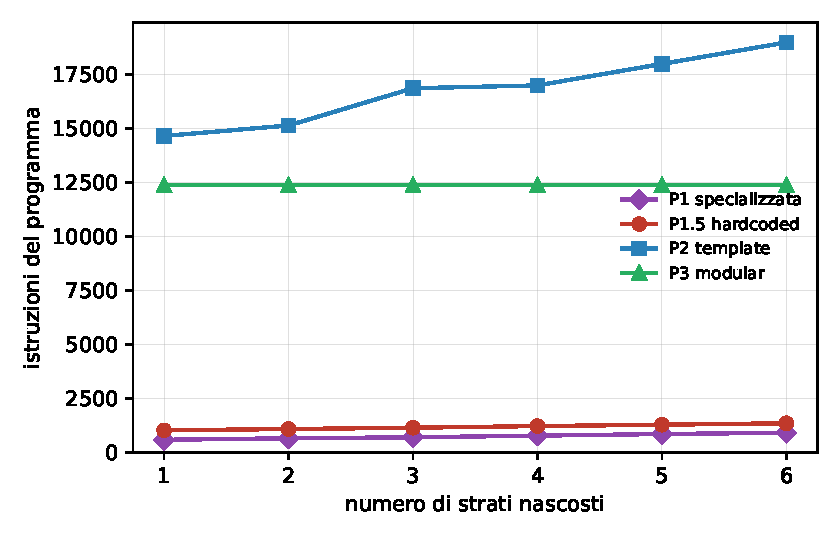
\includegraphics[width=0.92\textwidth]{figures/scaling_depth_insns.pdf}
\end{center}

\begin{lezione}
\textbf{P3 ha la stessa dimensione da uno a sei strati}: 12\,288 istruzioni in
ogni punto. \textbf{P2 cresce} di circa 870 istruzioni per strato, da 14\,604 a
18\,937.
\end{lezione}

P3 srotola \emph{un} solo strato denso generico e ci rientra a ogni passo della
rete, quindi la profondità non entra nel programma. P2 deve srotolarli tutti,
perché è un programma solo; ci riesce fino a venti strati grazie alla ReLU
senza bivio (capitolo \ref{ch:relu}).

\begin{center}
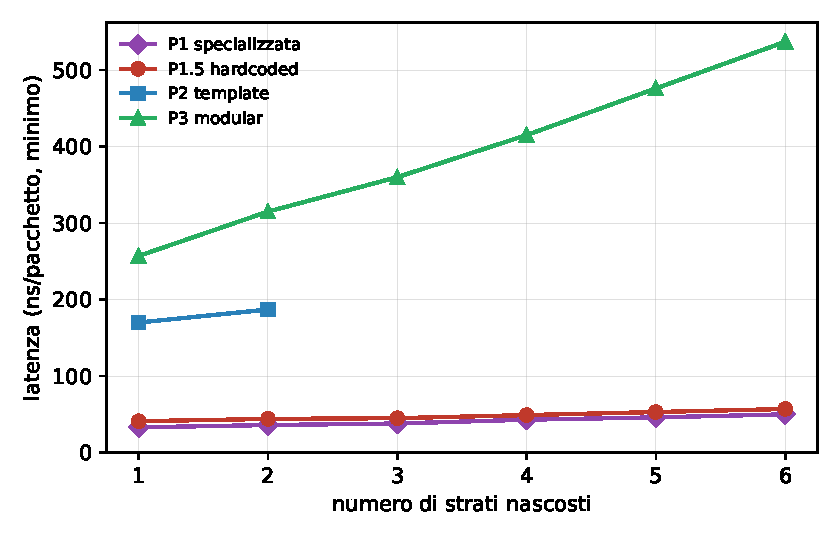
\includegraphics[width=0.92\textwidth]{figures/scaling_depth_latency.pdf}
\end{center}

\begin{lezione}
\textbf{E P3 lo paga in tempo: circa 53 nanosecondi per strato} (260 $\to$ 524~ns
da uno a sei strati), a istruzioni identiche. \textbf{P2 ne paga circa 26}
(171 $\to$ 300~ns): lo strato in più è codice in linea, niente salti e niente
letture per ricostruire il contesto. Le due P1 crescono di circa 6~ns per strato
(33 $\to$ 61 la specializzata, 40 $\to$ 67 la P1.5). Sul traffico vero lo stesso
andamento: P3 circa 60~ns per strato (capitolo \ref{ch:reale}).
\end{lezione}

Le due figure hanno la \emph{stessa} causa vista dai due lati. P3 è più piccolo
\textbf{perché} riusa un pezzo, ed è più lento \textbf{perché} riusarlo costa
un salto e delle letture ogni volta. È il compromesso della modularità, ridotto
a due numeri. La differenza vera sulla profondità resta un'altra: P3 cambia
profondità senza ricompilare, P2 deve ricompilare il programma.

\section{Aggiornare il modello: millisecondi per tutte}

\begin{center}
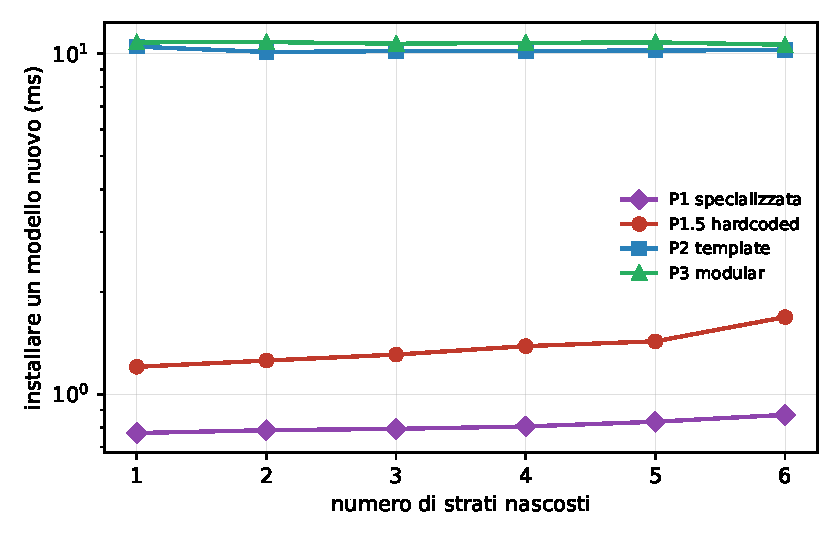
\includegraphics[width=0.92\textwidth]{figures/scaling_depth_update.pdf}
\end{center}

\begin{lezione}
Con P1 costruita come oggetto precompilato, installare un modello nuovo su un
nodo già in servizio costa \textbf{0,4--2,2 millisecondi} in P1 --- il nodo apre
e carica un file pronto --- e \textbf{10--12 millisecondi} in P2 e P3, che
scrivono in una tabella (pesi e semantica delle classi).

Contando anche il lavoro di P1 fuori dal nodo --- generare il C, compilarlo con
clang --- si sta fra 57 e 121~ms. P2 e P3 compilano con BCC una volta sola,
all'avvio del nodo (1,2--1,8~s), e mai più.
\end{lezione}

La differenza che resta fra le pipeline non è quindi il tempo di aggiornamento,
ma \emph{dove} serve il compilatore: P1 ne vuole uno per ogni modello nuovo, su
qualche macchina; P2 e P3 no.

\section{Larga o profonda? Dipende da chi la esegue}

Dato un numero di parametri da spendere, conviene metterli in \emph{un} layer
largo o in \emph{molti} stretti? È una domanda che si fa di solito parlando del
modello, come se la risposta fosse una proprietà della rete neurale. Qui non lo
è.

Cinque forme, tutte con lo stesso budget --- 592 pesi, con uno scarto del 2\%\
--- disposto in modo diverso: da un solo strato da otto neuroni a cinque strati
stretti.

\begin{center}
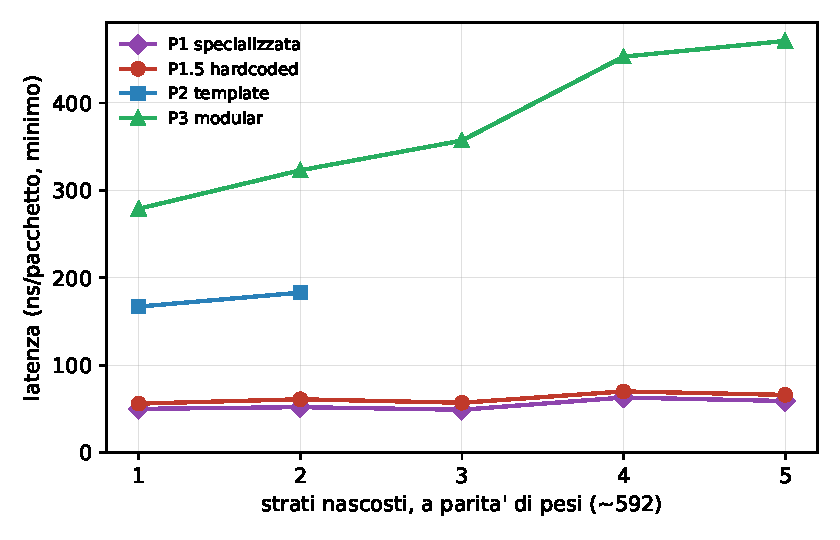
\includegraphics[width=0.92\textwidth]{figures/scaling_isoparam_latency.pdf}
\end{center}

\begin{lezione}
A parità di parametri le due versioni hardcoded cambiano poco e non in modo
monotono (54--68~ns la specializzata, 62--72 la P1.5). P2 perde il \textbf{53\%}
da uno a cinque strati (175 $\to$ 268~ns), P3 il \textbf{73\%} (284 $\to$ 490~ns).
Sul traffico vero P2 +35\% e P3 +60\%, con il costo fisso del nodo in più.

La stessa scelta di architettura costa poco o costa molto, a seconda della
pipeline su cui finisce.
\end{lezione}

\begin{center}
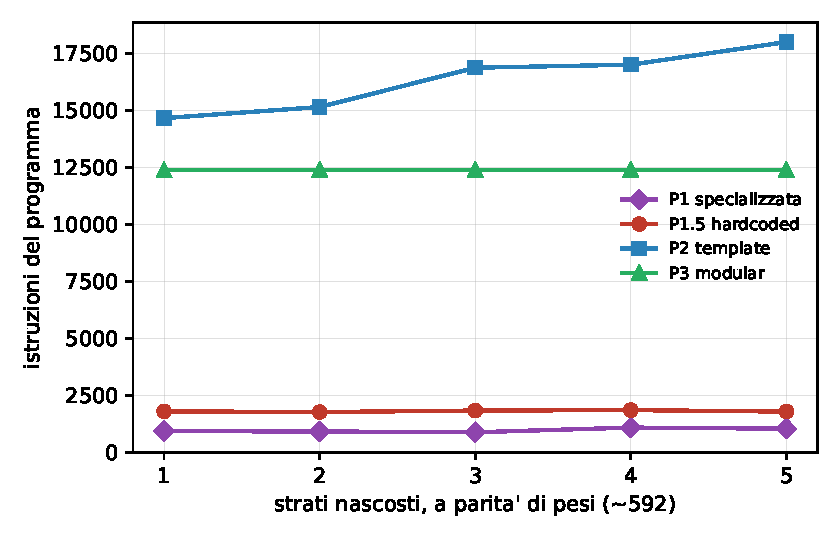
\includegraphics[width=0.92\textwidth]{figures/scaling_isoparam_insns.pdf}
\end{center}

P3 ha la riga \textbf{perfettamente orizzontale} --- 12\,288 istruzioni a tutti e
cinque i punti --- e perde comunque il 73\%\ di velocità.

\begin{lezione}
\textbf{Dimensione costante e tempo crescente} è la firma di un costo di
transizione, non di calcolo. In P3 si vede allo stato puro: ciò che cresce non è
il lavoro, è il numero di volte che il programma deve rientrare in sé stesso.
\end{lezione}

\subsection*{Con budget diversi, e ingressi diversi}

Il banco dedicato (\texttt{bench\_depth\_vs\_width}) prova tre budget e quattro
vettori d'ingresso, sulla sola P1:

\begin{center}
\small
\begin{tabular}{@{}lrrrr@{}}
\toprule
& \textbf{larga} & \textbf{2 strati} & \textbf{4 strati} & \textbf{8 strati} \\
\midrule
\multicolumn{5}{@{}l}{\emph{$\sim$300 pesi}} \\
ingresso con due one-hot (65 valori) & 39 ns & 44 & 48 & 62 \quad($+59\%$) \\
ingresso denso (11 valori)           & 93 ns & 90 & 85 & 83 \quad($-11\%$) \\
\addlinespace
\multicolumn{5}{@{}l}{\emph{$\sim$1\,200 pesi}} \\
ingresso con due one-hot (65 valori) & 105 ns & 145 & 165 & 211 \quad($+101\%$) \\
ingresso denso (11 valori)           & \emph{stack} & \emph{stack} & 330 & 295 \quad($-11\%$) \\
\bottomrule
\end{tabular}\\[2pt]
{\footnotesize\color{soft} P1 come oggetto AOT.
\emph{stack}: clang non compila, la forma chiede più dei 512 byte di stack di eBPF.}
\end{center}

Con un ingresso \textbf{grande e dominato da una one-hot} --- il caso di IPA, 52
dei 65 valori --- allargare batte approfondire, e a 1\,200 pesi la rete a otto
strati costa il doppio di quella larga. Con un ingresso \textbf{piccolo e
denso} vince la rete profonda: più veloce dell'11\% a 300 pesi e anche più
piccola (1\,323 contro 1\,490 istruzioni). Il motivo: una one-hot larga costa poco per pacchetto,
perché il datapath ne legge \emph{una colonna sola}; un ingresso denso invece fa
moltiplicare le letture per la larghezza del primo strato.

\subsection*{Il limite di P1 è lo stack}

Con la ReLU senza bivio (capitolo \ref{ch:relu}) il verificatore accetta tutto il
tier da $\sim$1\,200 pesi sull'ingresso di IPA. Il limite che resta non è del
verificatore: lo \textbf{stack} di eBPF, 512 byte. Con l'ingresso denso a 1\,200
pesi la forma larga (un solo strato da 63 neuroni) e quella a due strati da 26
chiedono più spazio per i valori intermedi di quanto il programma ne abbia, e
clang si ferma prima di produrre l'oggetto. A $\sim$4\,700 pesi succede a tutte
le forme.

\begin{lezione}
La frase giusta non è "le reti larghe sono preferibili a quelle profonde". È:
\emph{con un ingresso dominato da feature one-hot, allargare batte
approfondire; con un ingresso piccolo e denso vince la rete profonda; e oltre
qualche centinaio di pesi, in P1, è la forma larga a esaurire per prima lo
stack.}
\end{lezione}

\section{Congelare il nodo: conviene?}

L'indice del nodo è una \textbf{costante del deployment}: un nodo non cambia di
posto. Il codice però lo legge a runtime, e per farlo porta uno switch con un
caso per ogni nodo della rete --- 52 casi per Germany50, di cui ne esegue
\emph{uno}.

Congelandolo a tempo di generazione lo switch sparisce, e con lui la lettura
della tabella. Restano quattro numeri costanti, che il compilatore può piegare
dentro al conto.

\begin{center}
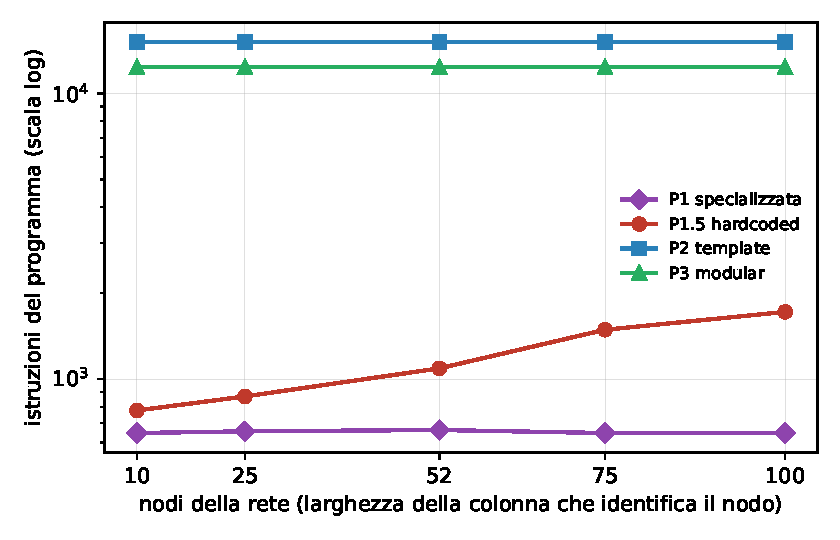
\includegraphics[width=0.92\textwidth]{figures/scaling_nodes_insns_log.pdf}
\end{center}

\begin{lezione}
La taglia della rete entra nel programma \textbf{solo} nella P1.5, che passa da
731 a 1\,673 istruzioni fra 10 e 100 nodi.

Congelando il nodo quella dipendenza \textbf{sparisce}: la riga della
specializzata è piatta, fra 602 e 618 a qualunque taglia.
\end{lezione}

(La scala è logaritmica: in lineare le due righe P1 resterebbero schiacciate
contro le quindicimila di P2.)

\subsection*{E la velocità}

\begin{center}
\small
\begin{tabular}{@{}lrrrrr@{}}
\toprule
\textbf{nodi} & 10 & 25 & 52 & 75 & 100 \\
\midrule
P1 specializzata & 40 & 40 & 41 & 42 & 39 ns \\
P1.5 hardcoded   & 46 & 45 & 46 & 47 & 46 ns \\
\bottomrule
\end{tabular}
\end{center}

La specializzata è più veloce di 4--7~ns, l'11--15\%, a ogni taglia: la lettura
della tabella del nodo e lo switch costano poco, ma si vedono. Entrambe sono
piatte: a runtime lo switch è un salto indicizzato, qualunque sia il numero dei
casi.

\begin{lezione}
Il motivo per cui la \emph{dimensione} crolla e il \emph{tempo} cala poco è lo
stesso: lo switch ha 52 casi ma ne esegue uno. Quelle 208 assegnazioni sono
compilate per eseguirne quattro. Toglierle libera molto \textbf{spazio} e un po'
di \textbf{tempo}.
\end{lezione}

\subsection*{Il controllo, e perché ci si può fidare}

Come si fa a essere sicuri che il divario venga davvero dalla one-hot del nodo e
non da qualcos'altro? Si prende un vettore d'ingresso che la feature \emph{non}
la contiene:

\begin{center}
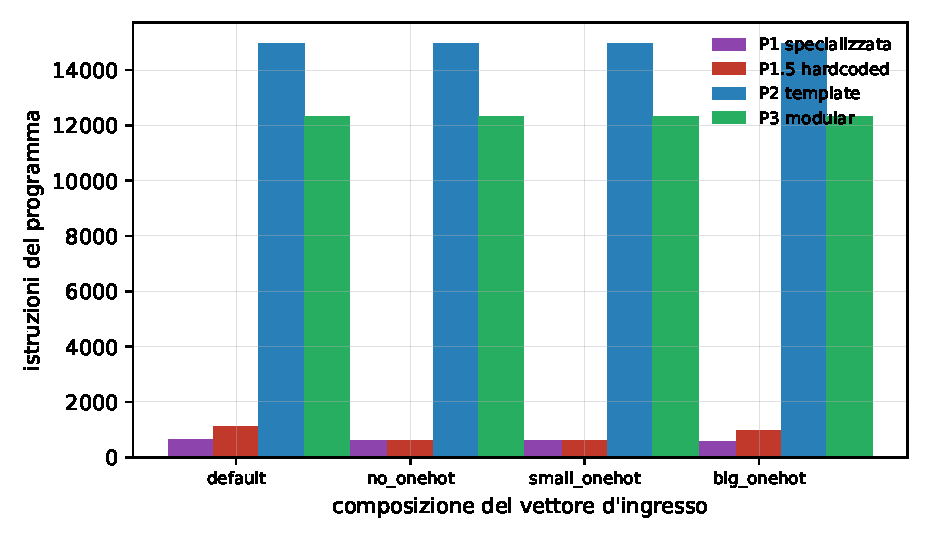
\includegraphics[width=0.92\textwidth]{figures/scaling_descriptor_insns.pdf}
\end{center}

Nelle due composizioni senza la feature \texttt{node} le due P1 sono
\textbf{identiche alla cifra} (611 e 611; 604 e 604). In quelle che ce l'hanno,
divergono. Il divario è tutto lì e nient'altro.

C'è poi una verifica che viene prima di ogni numero. Congelare il nodo significa
scegliere \emph{una colonna} della matrice dei pesi al momento di generare il
codice: sceglierne una sbagliata darebbe un programma più piccolo, più veloce, e
che calcola \textbf{un altro modello}. Ottanta casi, dieci valori di TTL per otto
configurazioni di link: la versione congelata decide sempre la stessa classe di
quella che legge il nodo dalla tabella.

\subsection*{I due vantaggi non si sommano}

\begin{center}
\small
\begin{tabular}{@{}lrrrrr@{}}
\toprule
\textbf{pesi a zero} & 0\%\ & 25\%\ & 50\%\ & 75\%\ & 90\%\ \\
\midrule
P1 specializzata & 618 & 564 & 484 & 401 & \textbf{243} \\
P1.5 hardcoded   & 1\,045 & 923 & 840 & 672 & \textbf{337} \\
\bottomrule
\end{tabular}
\end{center}

Al 90\%\ di zeri il divario scende da 427 a 94 istruzioni. Sparsità e nodo congelato sono
\textbf{due strade alla stessa riduzione}: se i pesi sono già quasi tutti zero,
il compilatore cancella lo switch da solo e non resta niente da congelare.

\subsection*{Le quattro risposte in una figura}

\begin{center}
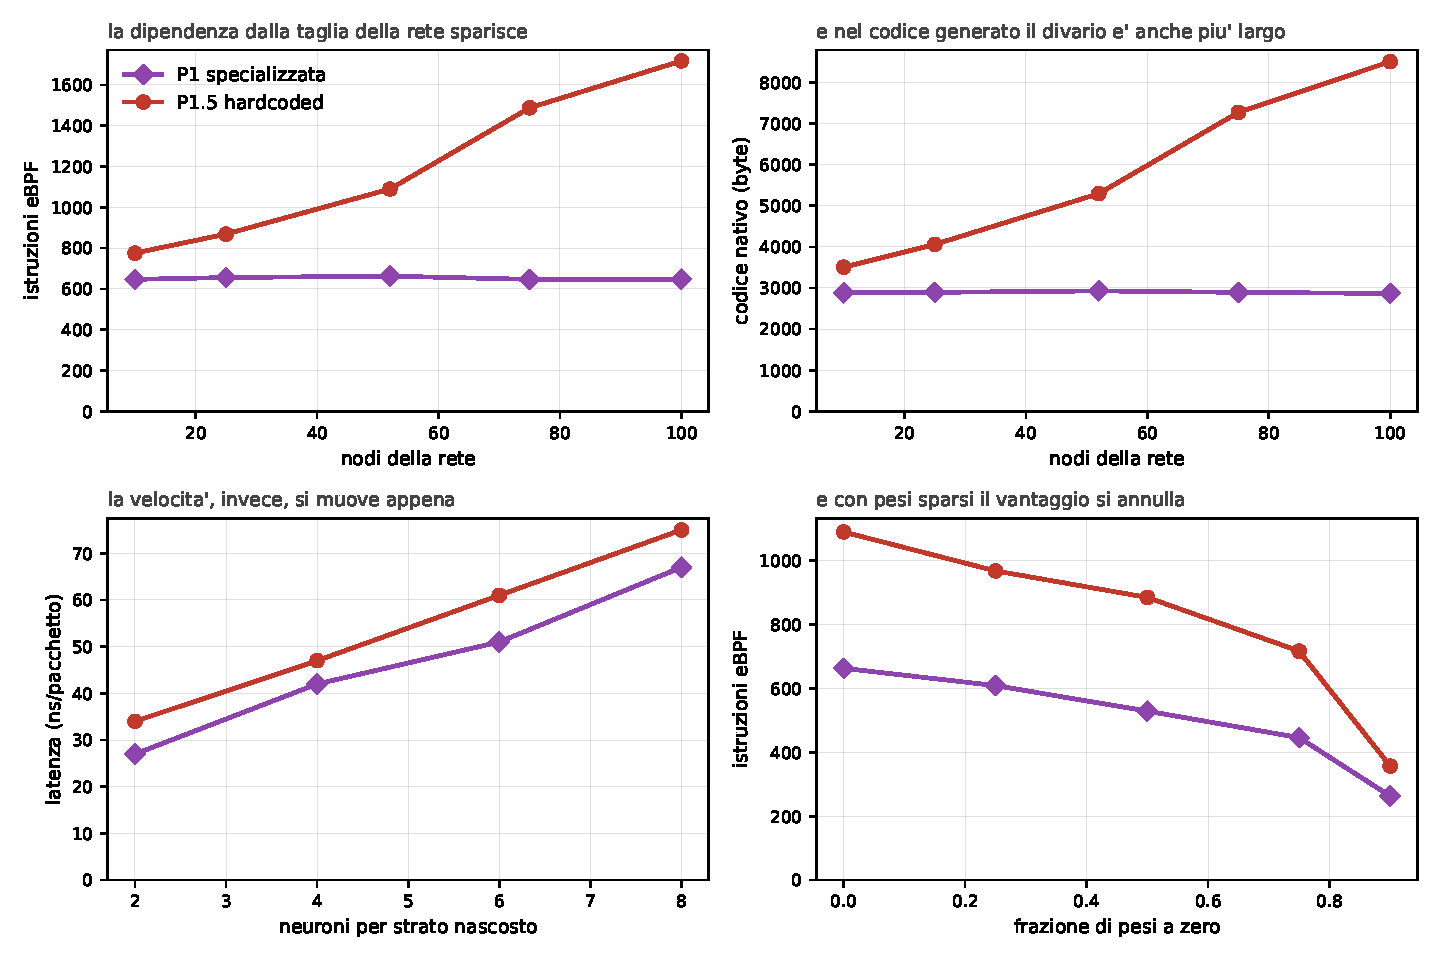
\includegraphics[width=\textwidth]{figures/duel_p1_vs_p15.pdf}
\end{center}

Qui ci sono solo le due P1: in tutte le altre figure P2 e P3 stanno un ordine di
grandezza più su e schiacciano questo confronto sul fondo del grafico. La
dimensione crolla e smette di dipendere dalla rete; il codice nativo crolla ancora
di più (2\,692 byte contro 8\,325 a cento nodi); la velocità migliora di poco; e
con i pesi sparsi le due curve si toccano.

\subsection*{Il verdetto}

\begin{lezione}
Congelare il nodo \textbf{non è soprattutto un'ottimizzazione di velocità}. È ciò
che rende la pipeline hardcoded \emph{praticabile su una rete grande}.

Lo switch della P1.5 cresce col numero di nodi moltiplicato per la larghezza del
primo strato. Su una topologia da 500 nodi con 8 neuroni sarebbero quattromila
assegnazioni srotolate, e c'è una taglia oltre la quale quel programma non si
carica più. La specializzata non ci arriva mai.

Il prezzo è \textbf{un binario per nodo}: 52 compilazioni (circa 70~ms ciascuna)
e 52 installazioni.
\end{lezione}

\section{Congelare quali porte esistono}

La sezione precedente congela \emph{dove} il nodo si trova. Questa congela
\emph{quante interfacce ha}.

Il modello riserva sei colonne per \texttt{link\_state} perché sei è il grado
del nodo più connesso della rete. Ma su un nodo di grado 3 le tre colonne
restanti non sono link caduti: dietro non c'è alcuna interfaccia. Valgono zero,
sempre.

\begin{lezione}
Non si congela il \textbf{valore} della feature, si congela la sua
\textbf{struttura}. Se un link sia su o giù resta letto a runtime; quello che
diventa noto alla compilazione è \emph{quali posizioni possono esistere}.
\end{lezione}

Il generatore non emette le colonne che restano fuori. Il termine che sparisce è
$\texttt{link\_state}[i] \cdot w[j][i]$ con $\texttt{link\_state}[i]$ nullo: la
somma è fra interi a 64 bit, quindi togliere un addendo nullo non cambia un bit.

\begin{center}
\small
\begin{tabular}{@{}lrrrrr@{}}
\toprule
\textbf{porte presenti} & 2 & 3 & 4 & 5 & 6 \\
\midrule
istruzioni eBPF & \textbf{534} & 554 & 570 & 594 & 618 \\
latenza         & 37 & 38 & 39 & 39 & 40 ns \\
\bottomrule
\end{tabular}
\end{center}

\textbf{Circa 21 istruzioni per porta}, in modo lineare, e \textbf{3~ns} fra grado
6 e grado 2, con la latenza che sale in modo monotono. Diversamente dal nodo, qui le
moltiplicazioni tolte vengono eseguite davvero a ogni pacchetto, e la misura le
vede: circa un nanosecondo per porta.

Le altre tre pipeline, che non specializzano niente, restano ferme lungo l'asse
(1\,045, 15\,089 e 12\,288 istruzioni, latenze piatte): la pendenza della
specializzata viene dalle porte e da nient'altro.

\subsection*{Il controllo, che è servito davvero}

Ottanta casi --- dieci valori di TTL per otto configurazioni di link
realizzabili --- danno la stessa classe fra la versione specializzata e quella a
larghezza piena. Ma quel numero, da solo, non dimostra niente: se quelle colonne
non spostassero mai la decisione, «le due versioni concordano» sarebbe vero anche
per una specializzazione \textbf{sbagliata}. Serve un controllo al contrario:
accendere uno slot che sul nodo non esiste, e pretendere che a quel punto le due
divergano. Su alcuni pesi quel controllo resta muto --- una colonna contribuisce
$1 \cdot w$ a un accumulatore che ne somma 65 --- e il banco cerca fra più semi
finché non morde: 29 divergenze.

\begin{lezione}
Un test che passa anche quando la sua ipotesi è violata non sta verificando
l'ipotesi.
\end{lezione}

\section{Due larghezze, due risposte opposte}

\begin{center}
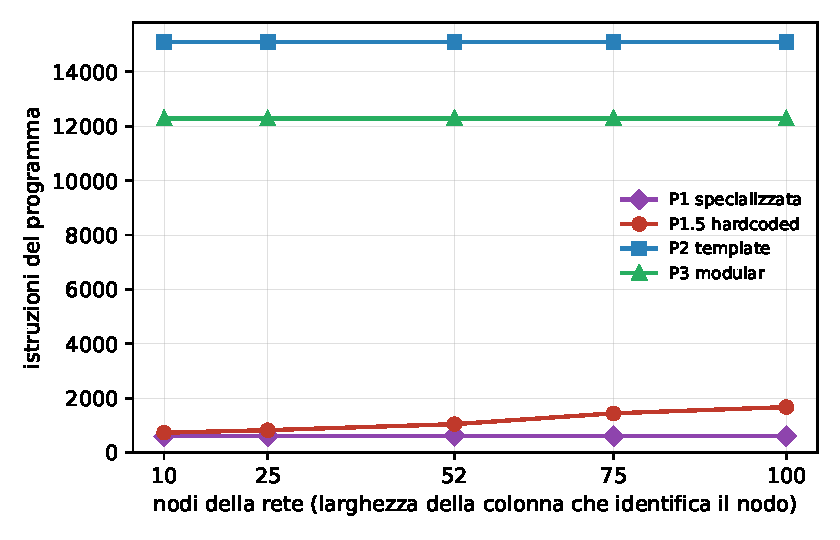
\includegraphics[width=0.92\textwidth]{figures/scaling_nodes_insns.pdf}
\end{center}

La taglia della \emph{rete} entra nel programma solo in P1.5: è lo switch della
one-hot che si srotola. P2 e P3 restano alla cifra esatta a ogni punto.

\begin{center}
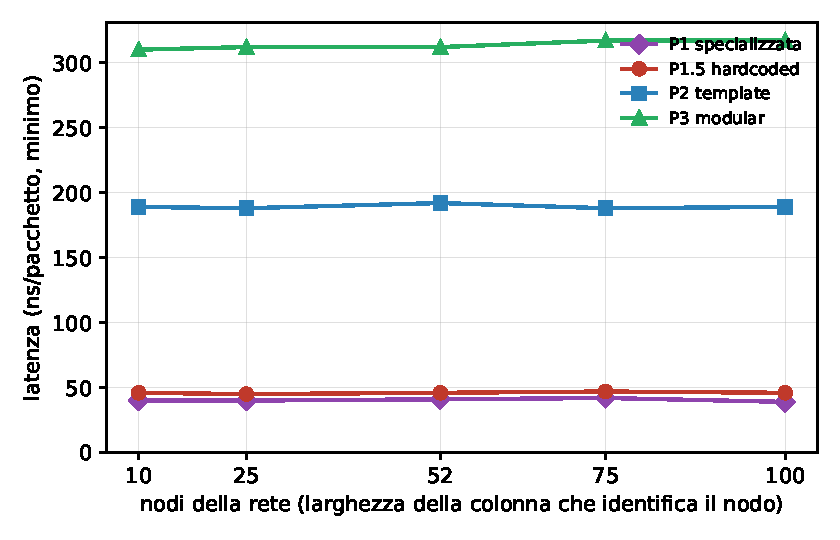
\includegraphics[width=0.92\textwidth]{figures/scaling_nodes_latency.pdf}
\end{center}

\textbf{Piatte tutte.} Cento nodi costano quanto dieci: una one-hot ha un solo
uno, quindi il datapath legge \emph{una sola colonna di pesi} qualunque sia la
larghezza del vettore.

Allargare i layer \emph{nascosti}, invece:

\begin{center}
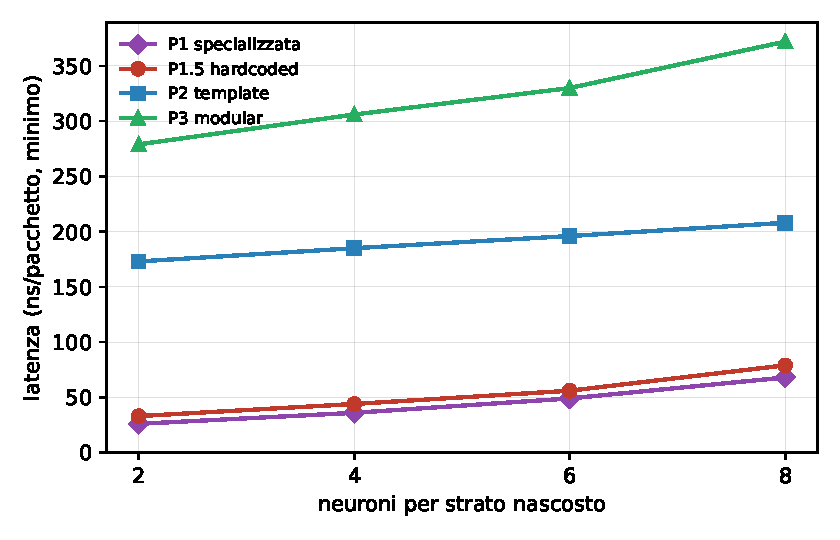
\includegraphics[width=0.92\textwidth]{figures/scaling_width_latency.pdf}
\end{center}

Da 2 a 8 neuroni: P1 specializzata 26 $\to$ 68~ns, P1.5 34 $\to$ 75, P2 178 $\to$
216, P3 280 $\to$ 386. Sul traffico vero P1 104 $\to$ 145 e P3 391 $\to$ 496~ns
di CPU per pacchetto (capitolo \ref{ch:reale}).

\begin{lezione}
\textbf{La rete può crescere quanto vuole; il modello no.}
\end{lezione}

\section{I pesi contano, ma solo per una delle tre}

\begin{center}
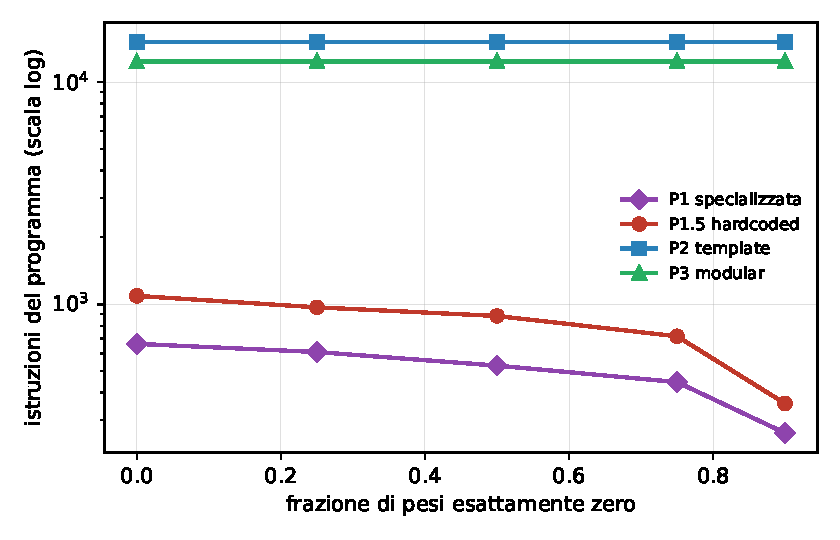
\includegraphics[width=0.92\textwidth]{figures/scaling_sparsity_insns_log.pdf}
\end{center}

\begin{lezione}
Con il 90\%\ dei pesi a zero, P1.5 passa da 1\,045 a \textbf{337 istruzioni} e
da 45 a 25~ns. P2 e P3 non si muovono di una istruzione, e di un paio di
nanosecondi al massimo. Sul traffico vero P1.5 scende da 120 a 106~ns di CPU,
P2 e P3 restano fermi.
\end{lezione}

P1 scrive i pesi nel codice come numeri, quindi il compilatore vede una
moltiplicazione per zero e la cancella. Per P2 e P3 uno zero è un byte in una
tabella come un altro. È l'unico asse su cui dimensione e tempo scendono
insieme.

\section{Che cosa questi grafici non dicono}

\begin{itemize}
\item Sono tutti \texttt{BPF\_PROG\_TEST\_RUN}: il programma, non il nodo sotto
      traffico. Gli stessi assi sotto traffico vero sono nel capitolo
      \ref{ch:reale}.
\item Oltre circa 115 nodi non si va senza alzare un tetto compilato e
      \textbf{rimisurare}.
\item Che i \emph{pesi}, a forma fissa, possano decidere se P1 si carica è
      possibile (il codice generato dipende dai valori), ma variando il solo seme
      dei pesi non è stato misurato. Con la ReLU senza bivio il verificatore ha
      molto margine (capitolo \ref{ch:relu}), quindi è poco probabile.
\end{itemize}

% ==================================================================
\chapter{Il costo del programma, misurato da solo}
\label{ch:programma}
% ==================================================================

Prima di mettere un programma in una rete conviene sapere quanto costa da solo.
Qui lo strumento è \texttt{BPF\_PROG\_TEST\_RUN}: il kernel esegue il programma
su un pacchetto preparato, in un ciclo, senza schede di rete, code o altri
programmi di mezzo. È come cronometrare un cassiere mentre batte sempre lo
stesso scontrino: misura il gesto, non la fila. La fila è l'argomento del
capitolo \ref{ch:reale}.

% ------------------------------------------------------------------
\section{La campagna sulle architetture}

Per rispondere a \emph{come cresce il costo quando il modello cresce} servono
più modelli misurati con la stessa metodologia: quattro assi, un solo parametro
che si muove per asse, minimo su sette prove.

\begin{center}
\small
\begin{tabular}{@{}llp{7.1cm}@{}}
\toprule
\textbf{Asse} & \textbf{Valori} & \textbf{Che cosa muove} \\
\midrule
\texttt{iv\_dense}   & $n_{in}$ 5, 9, 13, 17 &
  colonne d'ingresso tutte \emph{dense}: ognuna è letta da una mappa e
  moltiplicata \\
\texttt{iv\_onehot}  & $n_{in}$ 16, 32, 65 &
  colonne d'ingresso in una \emph{one-hot} \\
\texttt{width\_camp} & 65-$v$-$v$-7, $v$ 4, 8, 16, 32 &
  neuroni per strato nascosto \\
\texttt{depth\_camp} & 65-8$\ldots$8-7, 1--4 strati &
  profondità, a larghezza fissa 8 \\
\bottomrule
\end{tabular}
\end{center}

\subsection*{I muri, tutti dichiarati}

\textbf{Larghezza 16 e 32 su Pipeline 2 e 3.} I soffitti compilati valgono 8. E
Pipeline~3 non rifiuta il caricamento: risponde \texttt{XDP\_PASS} a runtime.
Una cella a larghezza 16 \emph{si caricherebbe, girerebbe, e restituirebbe una
latenza} --- di un programma che non calcola niente. Il banco controlla i
soffitti \emph{prima} di compilare e segna la cella \textsc{rifiutato}.

\textbf{Larghezza 32 su Pipeline 1.} La compilazione con clang fallisce (lo
stack di eBPF non basta). Ogni cella gira nel proprio sottoprocesso: la cella
esce \textsc{crash} e lo sweep continua. P1 a larghezza 16 carica (166--171~ns),
e P2 carica tutti i punti di \texttt{depth\_camp}, grazie alla ReLU senza bivio
(capitolo \ref{ch:relu}).

% ------------------------------------------------------------------
\section{Il problema: le MAC nominali non predicono la latenza}

Il modo naturale di mettere in relazione complessità e tempo è contare le
moltiplicazioni-accumulo dalla forma del modello: $n_{in} \times h_1$ per il
primo strato, e così via. Fatto così, non funziona: con le MAC nominali
sull'asse delle ascisse la retta spiega il 63\% della varianza per la P1
specializzata, il 24\% per P2 e il 10\% per P3.

Il sintomo più chiaro sta sull'asse \texttt{iv\_onehot}, dove il vettore
d'ingresso quadruplica:

\begin{center}
\small
\begin{tabular}{@{}rrrrrr@{}}
\toprule
$n_{in}$ & \textbf{pesi} & \textbf{p1\_static} & \textbf{hardcoded} &
\textbf{template} & \textbf{modular} \\
\midrule
16 & 271 & 65 ns & 65 ns & 169 ns & 361 ns \\
32 & 399 & 63 ns & 63 ns & 168 ns & 364 ns \\
65 & 663 & 64 ns & 64 ns & 170 ns & 367 ns \\
\bottomrule
\end{tabular}
\end{center}

$n_{in}$ per quattro, pesi per 2,4, e la latenza \textbf{non si muove su
nessuna delle quattro}. Le istruzioni di Pipeline~1 intanto salgono da 1\,099 a
1\,587: la taglia statica cresce, il percorso eseguito no.

\section{La soluzione: contare le MAC che vengono eseguite}

La causa è nel datapath, ed è una riga sola. Il ramo che tratta una feature
one-hot è questo:

\begin{lstlisting}[language=C]
} else if (code == FEAT_INGRESS_IF) {
    if (_raw_iface >= 1 && _raw_iface <= sz) {
        __u32 c = coff + (_raw_iface - 1);
        for (int j = 0; j < ML1_MAX_H1; j++)
            out[j] += LW_W(LW, woff + j * n_in + c);
    }
}
\end{lstlisting}

Una one-hot occupa \texttt{sz} colonne nella matrice dei pesi, ma nel datapath
ne attiva \emph{una}: il costo è $h_1$ addizioni, e non dipende da
\texttt{sz}. Contarla come $sz \times h_1$ moltiplicazioni sovrastima, e di
quanto dipende da quanta one-hot c'è nell'ingresso --- cioè cambia da asse ad
asse.

Il banco calcola quindi due colonne: \texttt{macs}, nominali, e
\texttt{macs\_eff}, che conta le one-hot per quello che eseguono. Con la
seconda sull'asse delle ascisse:

\begin{center}
\small
\begin{tabular}{@{}lrrrr@{}}
\toprule
& \multicolumn{2}{c}{\textbf{MAC eseguite}} &
  \multicolumn{2}{c}{\textbf{MAC nominali}} \\
\cmidrule(lr){2-3}\cmidrule(lr){4-5}
\textbf{Pipeline} & \textbf{ns/MAC} & \textbf{$r^2$} &
\textbf{ns/MAC} & \textbf{$r^2$} \\
\midrule
p1\_static & 0,287 & \textbf{0,99} & 0,071 & 0,63 \\
hardcoded  & 0,292 & \textbf{0,98} & 0,076 & 0,69 \\
template   & 0,574 & 0,71          & 0,092 & 0,24 \\
modular    & 1,195 & \textbf{0,92} & 0,106 & 0,10 \\
\bottomrule
\end{tabular}
\end{center}

Per Pipeline~3 si passa da $r^2 = 0{,}10$ a $r^2 = 0{,}92$, e
\texttt{p1\_static} da $0{,}63$ a $0{,}99$. Quattro assi costruiti in modi
diversi collassano sulla stessa retta, una per pipeline. P2 si ferma a
$r^2 = 0{,}71$: ha un costo fisso grande rispetto alla pendenza, e il suo
residuo più grande sta sull'asse della larghezza, dove i neuroni oltre la
larghezza del modello vengono calcolati comunque fino al soffitto compilato.

\begin{lezione}
\textbf{Il costo per MAC eseguita è una proprietà misurabile della pipeline}:
circa 0,29~ns quando i pesi sono compilati come letterali, circa 1,2~ns quando
vengono letti da una tabella (P3). Un fattore $4{,}2\times$: il prezzo della
genericità espresso in una costante invece che in un aneddoto.
\end{lezione}

Il pavimento della \texttt{baseline}, che di MAC ne esegue zero, sta a 14--15~ns: è il costo del framework XDP che ogni pipeline paga prima di moltiplicare
qualunque cosa.

% ------------------------------------------------------------------
\section{Due banchi, lo stesso programma, lo stesso numero}

I due banchi a \texttt{BPF\_PROG\_TEST\_RUN} misurano lo stesso programma, e
devono dare lo stesso numero. Sul modello 65-4-4-7:

\begin{center}
\small
\begin{tabular}{@{}lrrr@{}}
\toprule
\textbf{Pipeline} & \textbf{\texttt{test\_suite}} & \textbf{campagna} &
\textbf{scarto} \\
\midrule
baseline   &  14 ns &  14 ns & $0\%$ \\
hardcoded  &  52 ns &  45 ns & $-13\%$ \\
template   & 194 ns & 187 ns & $-4\%$ \\
modular    & 318 ns & 308 ns & $-3\%$ \\
\bottomrule
\end{tabular}
\end{center}

Concordano entro qualche nanosecondo, e i programmi non sono identici:
\texttt{test\_suite} usa i pesi veri del modello (1\,019 istruzioni per P1), la
campagna pesi sintetici a sparsità nulla (1\,045).

\subsection*{Il dettaglio che lo rende vero: un pacchetto nuovo ogni 200 giri}

Il kernel, dentro \texttt{BPF\_PROG\_TEST\_RUN}, non ripristina il pacchetto fra
una ripetizione e l'altra. Il datapath decrementa il TTL: riusando lo stesso
pacchetto, dopo una quarantina di esecuzioni il TTL resterebbe inchiodato a~1, e
da lì in poi ogni ripetizione prenderebbe il ramo

\begin{lstlisting}[language=C]
if (ip->ttl <= 1) { /* ... */ return XDP_PASS; }
\end{lstlisting}

che sta \textbf{dopo} l'inferenza --- il modello girerebbe comunque, e le curve
scalerebbero in modo regolare --- ma salta la coda di inoltro: decremento,
checksum, contatori, \texttt{mac\_table}, \texttt{bpf\_redirect}. Tutti i banchi
rinfrescano quindi il pacchetto ogni 200 esecuzioni partendo da TTL~255
($255 - 200 = 55$): nessuna ripetizione arriva alla scadenza.

\begin{lezione}
Un difetto che lascia il modello girare è il più difficile da vedere: le curve
restano belle. Si vede solo confrontando due banchi che devono dare lo stesso
numero.
\end{lezione}

% ------------------------------------------------------------------
\section{Il programma sul percorso vero: tre marcature}

Con traffico vero si può cronometrare il programma \emph{dentro} il percorso:
il dispatcher marca $T_1$ all'ingresso, il programma marca $T_2$ subito prima di
inoltrare, il contatore all'altro capo marca $T_3$.

\begin{center}
\small
\begin{tabular}{@{}lrrrrr@{}}
\toprule
& \textbf{baseline} & \textbf{P1} & \textbf{P1.5} & \textbf{P2} & \textbf{P3} \\
\midrule
$T_2-T_1$ (il programma) & 26 ns & 60 & 69 & 216 & 331 \\
$T_3-T_2$ (redirect, veth, ricezione) & 206 & 207 & 208 & 218 & 222 \\
$T_3-T_1$ a 50\,000 pacchetti/s & 221 & 259 & 274 & 442 & 609 \\
\bottomrule
\end{tabular}
\end{center}

Con \texttt{xdp\_gen}, nodo su un P-core. $T_2-T_1$ è piatto sul carico, da 0,5
a 3 milioni di pacchetti al secondo; $T_3-T_2$ è un costo comune di circa
210~ns che non dipende dalla pipeline; $T_3-T_1$ a basso carico è la latenza
minima dall'arrivo alla ripartenza. Sopra la baseline il solo programma costa
+34 / +43 / +190 / +305~ns. Su un E-core $T_2-T_1$ vale 28 / 72 / 84 / 266 /
434~ns e $T_3-T_2$ circa 245. La versione strumentata aggiunge due letture
dell'orologio per pacchetto: se qualcosa, questi numeri sono gonfiati. E il
throughput di questa versione non è una capacità: l'uscita resta sullo stesso
core del nodo.

% ==================================================================
\chapter{Il test reale: quanto costa un pacchetto al nodo}
\label{ch:reale}
% ==================================================================

\section{La domanda, in parole semplici}

Un nodo della rete riceve pacchetti, per ognuno esegue la rete neurale, decide
da quale porta farlo uscire, e lo spedisce. La domanda è: \textbf{quanti
pacchetti al secondo regge il nodo}, e \textbf{quanto tempo spende su ognuno}?

\begin{prima}[Un'immagine per tutto il capitolo: la cassa del supermercato]
Il nodo è un \textbf{cassiere}. I pacchetti sono i \textbf{clienti}. Il
generatore di traffico è la porta da cui entrano i clienti, e il collegamento
virtuale fra generatore e nodo è il \textbf{nastro} su cui i clienti aspettano:
ha 256 posti, e quando è pieno chi arriva viene mandato via.

Per sapere quanto spende il cassiere per cliente si fanno arrivare più clienti di
quanti ne riesca a servire, così che il nastro non sia mai vuoto, e si conta
quanti ne serve in un secondo. Se ne serve 5 milioni al secondo, spende
$1/5\,000\,000$ di secondo a cliente, cioè 200 nanosecondi.
\end{prima}

\section{Com'è fatto il banco}

Tutto sta sulla macchina di laboratorio, e ogni parte ha il suo core fisico, a
frequenza fissa (capitolo \ref{ch:macchina}):

\begin{center}
\begin{tikzpicture}[
  node distance=5mm,
  box/.style={draw=rule,fill=boxbg,rounded corners=2pt,minimum height=11mm,
              text width=22mm,align=center,inner sep=4pt,font=\small},
  dut/.style={box,fill=accent!12,draw=accent,thick},
  arr/.style={-{Stealth[length=5pt]},draw=soft,thick},
  lab/.style={font=\scriptsize\color{soft},align=center}
]
\node[box] (g) {generatore\\\footnotesize(\texttt{xdp\_gen}, CPU 10)};
\node[box,right=10mm of g,text width=16mm] (c1) {coda\\\footnotesize 256 posti};
\node[dut,right=10mm of c1] (n) {\textbf{nodo}\\\footnotesize programma XDP\\(CPU 6)};
\node[box,right=10mm of n,text width=16mm] (c2) {coda\\\footnotesize d'uscita};
\node[box,right=10mm of c2] (r) {nodo successivo\\\footnotesize(contatore, CPU 8)};
\draw[arr] (g) -- (c1);
\draw[arr] (c1) -- (n);
\draw[arr] (n) -- (c2);
\draw[arr] (c2) -- (r);
\node[lab,below=2mm of c1] {se è piena:\\\textbf{respinto}};
\node[lab,above=2mm of n] {ciò che misuriamo};
\end{tikzpicture}
\end{center}

\begin{itemize}
  \item \textbf{Il generatore} (\texttt{xdp\_gen}, sezione~\ref{sec:generatori})
        crea pacchetti uguali a quelli veri: stesso formato, stesso header IPA,
        stesso modello da eseguire. Un thread, che scrive nell'unica coda del nodo.
        Generatore e nodo successivo stanno su P-core; il nodo su un P-core, un
        E-core o un LP E-core, secondo la domanda (sezione~\ref{sec:corelenti}).
  \item \textbf{La coda d'ingresso} è quella di un \emph{veth}, il cavo virtuale di
        Linux: 256 posti, e la dimensione non si può cambiare.
  \item \textbf{Il nodo} è una delle pipeline caricata in XDP. È l'unica cosa che
        si vuole misurare.
  \item \textbf{Il nodo successivo} conta i pacchetti arrivati e li butta, su un
        core suo, così che sul core del nodo resti solo il lavoro del nodo.
\end{itemize}

Oltre alle cinque pipeline il banco misura, nella stessa sessione,
\textbf{\texttt{rxonly}}: un programma che prende il pacchetto dalla coda e lo
butta senza guardarlo. Dice quanto costa \emph{soltanto ricevere}: è il pavimento
sotto il quale nessuna pipeline può scendere.

\section{Come si misura, e perché così}

Un numero affidabile richiede quattro accortezze. Nessuna riguarda le pipeline:
senza, tutte farebbero sembrare il nodo diverso da com'è.

\subsection*{1. La finestra stazionaria}

Il banco avvia il generatore, aspetta che stia trasmettendo, lascia assestare la
coda, legge i contatori, aspetta 300~ms, li rilegge, e solo allora ferma il
generatore. Il rate è la differenza fra le due letture divisa per il tempo fra
le due letture: l'avvio e l'arresto restano fuori.

\subsection*{2. Letture brevi}

Ogni lettura (generatore più nodo) deve durare meno di 3~ms; se dura di più viene
rifatta, e le si attribuisce l'istante a metà. Un processo interrotto a metà
lettura attribuirebbe ai contatori un istante sbagliato di tutta l'interruzione.
Un test senza kernel lo verifica con un generatore simulato.

\subsection*{3. I respinti contano}

Quando la coda d'ingresso è piena il collegamento rifiuta il pacchetto
(«respinto»). Un pacchetto respinto è un pacchetto che il nodo non ha preso,
perché non svuotava la coda abbastanza in fretta: \textbf{è una perdita del
nodo}. Il banco conta separatamente i \textbf{respinti} (mai entrati) e i
\textbf{persi dopo l'ingresso} (entrati ma non usciti).

\subsection*{4. Il tempo di CPU, non il tempo che passa}

Il banco misura anche quanto il core del nodo è occupato, nella stessa finestra in
cui conta i pacchetti, e dà il costo come \textbf{tempo di CPU per pacchetto}:
occupazione per il tempo diviso i pacchetti. Se il nodo lavora il 100\% del tempo
coincide con 1 diviso la capacità; se a tratti aspetta, toglie l'attesa. Con
\texttt{xdp\_gen} il nodo lavora al 100\%, e le due misure coincidono.

Nella stessa lettura il banco legge anche i \textbf{contatori hardware} del core
del nodo: istruzioni e cicli. Divisi per i pacchetti dicono quante istruzioni
costa un pacchetto e quante ne esegue il core per ogni ciclo (l'IPC). Il tempo
di CPU dice \emph{quanto} costa un pacchetto; istruzioni e IPC dicono
\emph{perché}.

\section{Il generatore}
\label{sec:generatori}

\subsection*{\texttt{xdp\_gen}: pacchetti come da una scheda di rete}

Il generatore (\texttt{ipa/test/xdp\_gen.py}) consegna al cavo virtuale pacchetti
già nel formato di XDP, con \texttt{BPF\_PROG\_TEST\_RUN} in modalità \emph{live
frames}: il kernel li prepara in una sua riserva di pagine, con i 256 byte liberi
davanti che XDP vuole, e li spedisce davvero. Niente skb e niente copia: il
pacchetto arriva al nodo come arriverebbe da una scheda di rete con XDP nativo, e
il nodo paga solo il proprio lavoro. Un solo thread offre fino a circa 19 milioni
di pacchetti al secondo, ed è così che si usa: un thread per ogni coda del nodo
(sezione~\ref{sec:scrittore}).

Ogni misura è \textbf{una sola chiamata} al kernel, interrotta da un segnale a
fine finestra. Ogni chiamata, infatti, parte e finisce con una pausa del
generatore di circa 12~ms dentro il kernel: con più chiamate per finestra il
generatore tacerebbe una parte del tempo, e il nodo svuoterebbe la coda e
dormirebbe. Le statistiche di scheduling del thread del nodo lo controllano: a
coda piena lavora il 100\% del tempo.

\subsection*{Il ritmo e il timbro}

Per il test al crescere del traffico (sezione~\ref{sec:bitrate}) serve un ritmo
fissato, e \texttt{xdp\_gen} non ne ha uno suo: spinge al massimo. Il ritmo lo
tiene il suo programma, che a ogni giro guarda l'orologio: se non è ancora il
momento scarta il pacchetto (la pagina torna subito alla riserva) e riprova;
quando è il momento lo spedisce, e fissa il prossimo istante un intervallo più in
là. I pacchetti partono a distanza regolare, non a raffiche: una raffica da 256
riempirebbe da sola la coda e farebbe perdere pacchetti sotto capacità. Nello
stesso istante il programma scrive nel pacchetto un timbro con l'ora di partenza,
e il nodo successivo misura il ritardo. Il ritmo è esatto fino a circa 11 milioni
di pacchetti al secondo (a 12 ne parte il 98\%).

\subsection*{L'alternativa: \texttt{pktgen}}

\texttt{pktgen} è il generatore del kernel: fabbrica i pacchetti come lo stack di
rete, in una \emph{skb} con 64 byte liberi davanti, e il cavo virtuale li
\textbf{ricopia} in una pagina nuova prima di consegnarli al nodo. La copia la
paga il nodo, e su una scheda vera non esisterebbe.

Per questo il banco usa \texttt{xdp\_gen}, e tutte le cifre di questo capitolo
sono con \texttt{xdp\_gen}; \texttt{pktgen} resta disponibile per i percorsi che lo
richiedono.

\section{Perché un core vero, tutto suo}

Il nodo deve avere un core fisico suo, che non gli venga mai tolto, e il conto
che lo spiega è semplice. La coda d'ingresso ha 256 posti. A 1,5 milioni di
pacchetti al secondo un pacchetto arriva ogni $1/1{,}5\cdot10^6 \approx
0{,}67$~microsecondi, quindi la coda si riempie in
\[
  256 \times 0{,}67~\mu\text{s} \;\approx\; 170~\mu\text{s} .
\]
Se il core del nodo si ferma per più di 170 microsecondi --- perché il sistema
lo dà a un altro processo, o perché si addormenta --- la coda trabocca e i
pacchetti vengono respinti, \emph{per quanto veloce sia il programma}.
Nell'immagine del supermercato: il cassiere è bravissimo, ma se ogni tanto esce
dalla cassa per qualche secondo il nastro si riempie e i clienti vengono mandati
via. Una macchina virtuale, i cui core sono thread dell'ospite che possono
sparire per qualche millisecondo, non può fare questo banco.

Per questo:

\begin{itemize}
  \item \textbf{Core veri, ognuno col suo compito.} Generatore sul core 10, nodo
        sul core 6 (o 12, o 20), nodo successivo sull'8. Nessun altro processo,
        nessuna interruzione e nessun thread del kernel sul core del nodo
        (capitolo \ref{ch:macchina}).
  \item \textbf{Il core del nodo non dorme mai.} Gli stati di sonno profondi sono
        spenti: il risveglio dal più profondo costa 310 microsecondi, più dei 170
        che la coda concede. Sotto capacità il nodo non respinge niente.
  \item \textbf{Frequenza fissa e misurata}: 3\,472--3\,507~MHz sul core del nodo
        durante ogni misura di traffico (2\,500 sul LP E-core), letta dai
        contatori del processore.
  \item \textbf{Generatore e nodo su core separati}, quindi il generatore non è
        dentro la misura: il ritmo a cui il nodo satura è quello del nodo.
\end{itemize}

Il risultato si vede ripetendo: cinque giri allo stesso punto danno lo stesso
inoltro in genere entro lo 0,1\%, al massimo entro il 6\% vicino al punto in cui
la pipeline smette di reggere; la stessa pipeline misurata in quattro modi
diversi nella stessa sessione dà lo stesso costo entro il 2\%.

\section{I limiti del test, con esempi}
\label{sec:limiti}

Il condizionamento della macchina toglie il rumore. Non toglie i limiti di un
banco che sta tutto su un portatile: vanno conosciuti, perché ognuno dice quali numeri si possono citare
e quali no.

\subsection*{1. Il generatore può non bastare, o intralciare}

Se il nodo è più veloce di quanto il generatore riesca a produrre, il banco
misura il generatore. Un thread di \texttt{xdp\_gen} offre circa 19 milioni di
pacchetti al secondo a massima spinta, circa 12 a ritmo fissato e circa 9 a ritmo
fissato quando i pacchetti vengono inoltrati: per questo su un core
\texttt{rxonly} non arriva mai al suo limite, la baseline ci arriva appena, e
sulle curve del bit rate la baseline non lo raggiunge (da 9 milioni perde l'1\%
con il nodo al 60\%: è il banco, e il test lo riconosce dall'occupazione del
nodo). Aggiungere thread
sembra la soluzione, ma più thread che scrivono nella \emph{stessa} coda si
intralciano, e rallentano anche il nodo che la svuota: è la
sezione~\ref{sec:scrittore}.

\subsection*{2. Contare all'uscita può sottostimare il nodo}

Il nodo successivo, che conta i pacchetti arrivati, ha i suoi core e i suoi
tetti. Se si misura il nodo contando \emph{ciò che arriva dall'altra parte},
quando il nodo è più veloce dell'uscita si misura l'uscita.

\begin{prima}[Esempio: la baseline che sembrerebbe lenta]
Un core d'uscita spende circa 70~ns per ricevere, contare e restituire un
pacchetto: regge al più una dozzina di milioni di pacchetti al secondo. Se due
core del nodo gli mandano 25 milioni di pacchetti al secondo, la baseline ne
\emph{elabora} 25 ma all'altra parte ne arrivano 12; P2 ne elabora 6 e arrivano
tutti. Contando gli arrivi, la baseline sembrerebbe più lenta di P2 ---
impossibile, perché fa strettamente meno lavoro.

Per questo il controllo di validità del banco (``la baseline dev'essere la più
veloce'') conta i pacchetti \emph{elaborati dal nodo}, la stessa misura con cui
il banco calcola il costo, e non quelli arrivati all'uscita.
\end{prima}

Con un solo scrittore per coda anche all'uscita il nodo successivo tiene il passo:
con due core sul nodo serve una coda d'uscita per ciascun core, e un core d'uscita
per ciascuna coda; allora arrivano tutti, anche 29 milioni al secondo
(sezione~\ref{sec:duecore}).

\subsection*{3. Il cavo è virtuale, e tutto sta su un processore}

Il ``ricevere'' misurato è prendere il pacchetto dalla coda di un cavo virtuale,
non dalla memoria di una scheda di rete; ``inoltrare'' è accodarlo sul cavo
successivo, non scrivere un descrittore di trasmissione. Generatore, nodo e nodo
successivo sono core dello stesso chip e condividono cache e memoria. Il portatile
non ha una scheda di rete cablata che supporti XDP nativo.

Esempio: i 66~ns per pacchetto della baseline sono il prezzo \emph{di questo
percorso}. Su una scheda vera sarebbero altri numeri, e le cifre assolute di
questo capitolo con loro. I \textbf{confronti} fra pipeline no: il percorso è lo
stesso per tutte, e si sottrae.

\subsection*{4. Un solo tipo di pacchetto per volta}

In una misura tutti i pacchetti sono uguali: stesso modello, stesso TTL, stessa
classe decisa. Il processore impara in fretta un flusso così (il predittore dei
salti, la cache), e un traffico misto costerebbe un po' di più. Le classi si
misurano una alla volta, ed è così che si è visto che scartare costa più che
inoltrare.

\subsection*{5. Il ritardo a basso carico contiene il generatore}

\texttt{xdp\_gen} spedisce a lotti di 256 frame, e il nodo viene svegliato a fine
lotto: a basso carico un pacchetto può aspettare fino a una dozzina di
microsecondi prima che il nodo lo veda, e la mediana del ritardo, 17--19~µs sul
P-core, contiene quell'attesa. Lotti più piccoli la tolgono, ma il generatore
regge ritmi più bassi. Il salto del ritardo a coda piena, che è ciò che il test
cerca, non cambia.

\subsection*{6. Il punto esatto in cui comincia la perdita è instabile}

Al confine fra ``regge'' e ``perde'' basta un'esitazione di pochi microsecondi per
perdere un pacchetto: lo stesso punto, ripetuto, varia fino al 6\%, mentre la
saturazione varia di 1--3\%. Si citano quindi la saturazione e i gradini della
scala, non il confine esatto.

\subsection*{7. Il portatile scalda}

Oltre 3,5~GHz non regge una misura intera, e anche a 3,5 capita che il
processore nel suo insieme tocchi per un attimo la soglia di temperatura, di
solito mentre clang compila sugli altri core. Il banco lo registra e conta le
finestre disturbate (anche il funzionamento a batteria è un disturbo): nelle
misure di traffico di questo capitolo nessuna finestra ha avuto throttling, e
il core del nodo è rimasto a 3\,500~MHz.

\section{Il risultato: quanto regge il nodo}

Con \texttt{xdp\_gen}, un core del nodo (un P-core a 3,5~GHz), pacchetti da 64
byte, tre giri:

\begin{center}
\small
\begin{tabular}{@{}lrrrrrr@{}}
\toprule
\textbf{Pipeline} & \textbf{Mpps} & \textbf{ns per pacchetto} & \textbf{sopra la baseline}
& \textbf{cicli} & \textbf{istruzioni} & \textbf{IPC} \\
\midrule
solo ricezione (\texttt{rxonly}) & 19,47 & $\approx 41$ & --- & 161 & 384 & 2,4 \\
baseline (nessuna rete)  & 15,27 & 66 & --- & 225 & 606 & 2,7 \\
P1 statica               & 8,56 & 117 & $+51$ ns & 402 & 1\,220 & 3,0 \\
P1.5 (hardcoded)         & 8,04 & 124 & $+58$ ns & 432 & 1\,426 & 3,3 \\
P2 (template)            & 3,45 & 290 & $+224$ ns & 1\,013 & 4\,556 & 4,5 \\
P3 (modular)             & 2,36 & 425 & $+359$ ns & 1\,483 & 6\,573 & 4,4 \\
\bottomrule
\end{tabular}\\[2pt]
{\footnotesize\color{soft} Nodo occupato al 100\% (79\% per \texttt{rxonly}, che
non satura: il suo valore è indicativo). La baseline satura appena: il
generatore ne offre 15,3 milioni al secondo. Cicli e istruzioni sono per
pacchetto, dai contatori hardware del core del nodo.}
\end{center}

\begin{lezione}
La \textbf{baseline} riceve, legge l'intestazione, decrementa il TTL e inoltra.
Tutto ciò che le pipeline aggiungono sopra è \textbf{il costo della rete
neurale}: circa 50--60~ns quando i pesi sono scritti nel programma (P1, P1.5),
circa 225~ns quando la forma della rete è letta da una tabella (P2), circa 360~ns
quando anche la profondità lo è (P3).
\end{lezione}

Come si legge la colonna dei nanosecondi, con un esempio. La baseline regge
15,27 milioni di pacchetti al secondo, cioè spende $10^9 / 15{,}27 \cdot 10^6 =
66$~ns per pacchetto; P2 ne regge 3,45 milioni, cioè 290~ns. La differenza, $290
- 66 = 224$~ns, è il tempo che P2 spende a eseguire la rete neurale: tutto il
resto --- ricevere, leggere l'intestazione, inoltrare --- lo fanno tutte e due
allo stesso modo. I cicli confermano: a 3,5~GHz 66~ns sono 231 cicli, e il
contatore ne conta 225. P3 varia più delle altre fra una misura e l'altra: lo
stesso modello dà 416--445~ns nella stessa giornata.

Le istruzioni per pacchetto dicono un'altra cosa che il programma da solo non
dice: P3 \emph{esegue} più istruzioni di P2 (6\,573 contro 4\,556), pur
caricandone di meno. E l'IPC delle pipeline con i pesi in tabella è alto, oltre
4: è aritmetica in fila, senza bivi, che il core esegue molte istruzioni per
volta.

E sotto la capacità? Sulle curve del bit rate (sezione~\ref{sec:bitrate}), finché
il traffico resta sotto la capacità di una pipeline \textbf{nessun pacchetto
viene respinto} (al massimo lo 0,05\%). Un nodo sotto la sua capacità consegna
tutto.

\subsection*{P1 e P1.5 si separano}

8,56 contro 8,04 milioni al secondo: congelare il nodo vale circa 7 nanosecondi
sul percorso vero ($117$ contro $124$~ns per pacchetto), e 206 istruzioni in meno
per pacchetto. Piccolo, ma fuori dal rumore.

\subsection*{Da che cosa il costo non dipende}

\begin{itemize}
  \item \textbf{La taglia del pacchetto non conta}: a 64, 512 e 1\,514 byte il costo
        è lo stesso entro l'1\%. Il nodo guarda solo l'intestazione.
  \item \textbf{La porta d'uscita conta poco}: le cinque classi che inoltrano costano
        uguale entro il 2--3\% per P1, P1.5 e P3, entro il 12\% per P2.
  \item \textbf{Scartare costa di più che inoltrare}: la classe DROP costa circa
        50~ns in più delle altre (P1 166 contro 118--120, P1.5 176 contro
        124--127, P3 467 contro 416--426). Quando il pacchetto viene scartato la
        sua pagina di memoria si restituisce sul core del nodo; quando viene
        inoltrato, su quello del nodo successivo. È un effetto del banco, non
        della pipeline.
\end{itemize}

\section{Uno scrittore per coda}
\label{sec:scrittore}

Il generatore usa \textbf{un thread per coda} del nodo, e non di più. Più thread
che scrivono nella stessa coda da 256 posti devono passarsi un lucchetto e le
stesse righe di cache; il core del nodo, che dalla stessa coda legge, ne subisce
il rallentamento, e il nodo elabora \emph{meno} pacchetti invece di più. È come
una cassa dove tre fornitori scaricano merce nello stesso punto: il cassiere non
lavora peggio, ma gli spazi sono contesi. Il danno è grande per i programmi
leggeri e quasi nullo per quelli il cui limite è davvero il programma.

\begin{lezione}
Un solo scrittore per coda, in ingresso e in uscita: più thread di generatore
non aiutano, peggiorano. Con una scheda di rete vera la regola è rispettata da
sé: la coda di ricezione la riempie la scheda, un solo scrittore, e i pacchetti
degli altri host arrivano in fila sul cavo. Resta quello che conta, la coda
piena davanti a un nodo troppo lento.
\end{lezione}

\section{Al crescere del bit rate}
\label{sec:bitrate}

La domanda: al crescere del traffico offerto la coda si riempie, il
tempo di attraversamento cresce, e poi si perde. Se si perde \emph{all'ingresso}
del programma, il collo di bottiglia è il programma; se si perde \emph{dopo}, è
la trasmissione. Per saperlo bisogna contare quanti pacchetti il programma
riceve e quanti ne rilancia.

\subsection*{Due programmi sullo stesso aggancio}

Un'interfaccia porta un solo programma XDP. Due programmi sullo stesso aggancio
si ottengono in \textbf{catena}, con lo stesso salto fra programmi che le
pipeline usano già:

\begin{center}
\begin{tikzpicture}[
  box/.style={draw=rule,fill=boxbg,rounded corners=2pt,minimum height=9mm,
              inner sep=5pt,font=\scriptsize,align=center},
  arr/.style={-{Stealth[length=4pt]},draw=soft,thick}
]
\node[box] (g) {generatore\\(\texttt{xdp\_gen})};
\node[box,right=11mm of g,draw=accent] (c) {programma 1\\conta e basta\\\texttt{ing\_count += 1}};
\node[box,right=11mm of c,draw=accent] (p) {programma 2\\la pipeline};
\node[box,right=14mm of p] (n) {nodo successivo\\conta e misura\\il ritardo};
\draw[arr] (g) -- node[above,font=\scriptsize] {coda} (c);
\draw[arr] (c) -- node[above,font=\scriptsize] {salto} (p);
\draw[arr] (p) -- node[above,font=\scriptsize] {redirect} (n);
\end{tikzpicture}
\end{center}

Il primo programma è attaccato all'interfaccia, conta ogni pacchetto e salta al
secondo, che è il dispatcher della pipeline, identico a quello di produzione.

\textbf{Perché in catena.} Il kernel tiene, per ogni interfaccia, \emph{un}
programma XDP nell'aggancio nativo: è come è fatto XDP, non un limite di questo
progetto. I modi di averne più di uno sono tutti catene. Quello standard è
\texttt{libxdp}, che aggancia un programma \emph{dispatcher} con alcuni posti
liberi e ci inserisce gli altri; quello usato qui è il salto fra programmi
(\emph{tail call}) che le pipeline già usano, senza dipendenze in più. Il salto in
più costa da $-3$ a $+2$~ns, dentro la variazione fra le ripetizioni: il kernel
tiene il tempo di ogni programma attaccato, e lo si misura con e senza il
contatore davanti.

Così si hanno tre conteggi per ogni valore di traffico: \textbf{inviati} (dal
generatore), \textbf{ricevuti} (dal programma 1) e \textbf{inoltrati} (arrivati
al nodo successivo). Inviati meno ricevuti è la perdita \emph{prima} del
programma; ricevuti meno inoltrati quella \emph{dopo}. Un terzo metodo,
\texttt{rxonly}, è il contatore da solo: dice quanto regge la sola ricezione allo
stesso ritmo, e separa il collo del programma da quello del banco.

Il banco misura sedici valori di traffico, da 0,5 a 12 milioni di pacchetti al
secondo (da 0,26 a 6,1~Gbit/s a pacchetti da 64 byte), cinque giri ciascuno. Il
ritardo è quello di tutto il percorso: dal timbro che \texttt{xdp\_gen} scrive nel
pacchetto quando lo spedisce all'arrivo al nodo successivo.

\subsection*{Ricevuti e inoltrati}

\begin{center}
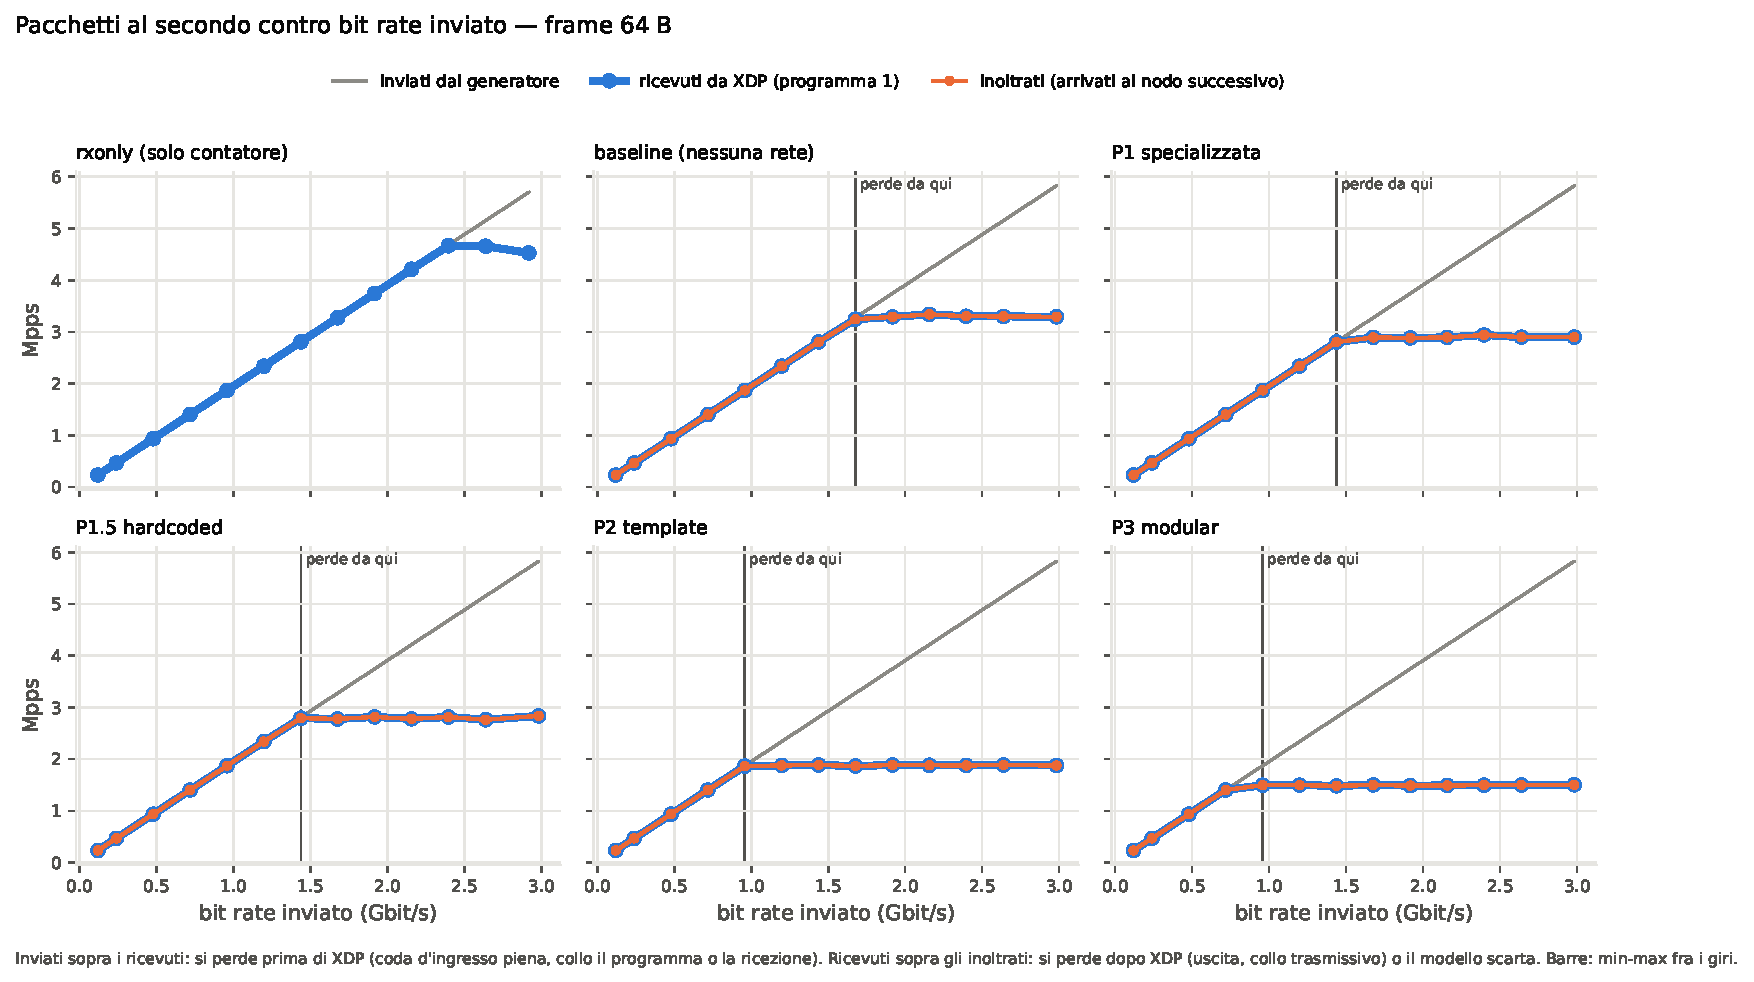
\includegraphics[width=\textwidth]{figures/bitrate_pps.pdf}
\end{center}

Ogni pannello ha tre curve. Finché il nodo regge sono sovrapposte: tutto ciò
che si invia viene ricevuto e inoltrato. Oltre il suo limite la linea grigia
(inviati) continua a salire e le altre due si fermano \textbf{insieme}, alla
capacità della pipeline: 8,66 milioni al secondo per P1, 8,17 per P1.5, 3,45 per
P2, 2,37 per P3, la stessa cifra del test di saturazione (8,56, 8,04, 3,45 e 2,36)
entro il 2\%; al ginocchio il nodo lavora il 99,5--100\% del tempo. La baseline è
un caso a parte: da 9 milioni al secondo perde circa l'1,3\%, ma con il nodo al
60\%. Il nodo ha tempo libero, quindi il limite è del banco: quando i pacchetti
vengono inoltrati \texttt{xdp\_gen} non ne manda più di circa 9 milioni al
secondo. La capacità della baseline resta quella del test di saturazione, 15,3
milioni. Che ricevuti e inoltrati restino sovrapposte è la risposta alla
domanda: \textbf{il programma rilancia tutto ciò che riceve}, e ciò che manca
non è mai entrato.

\begin{center}
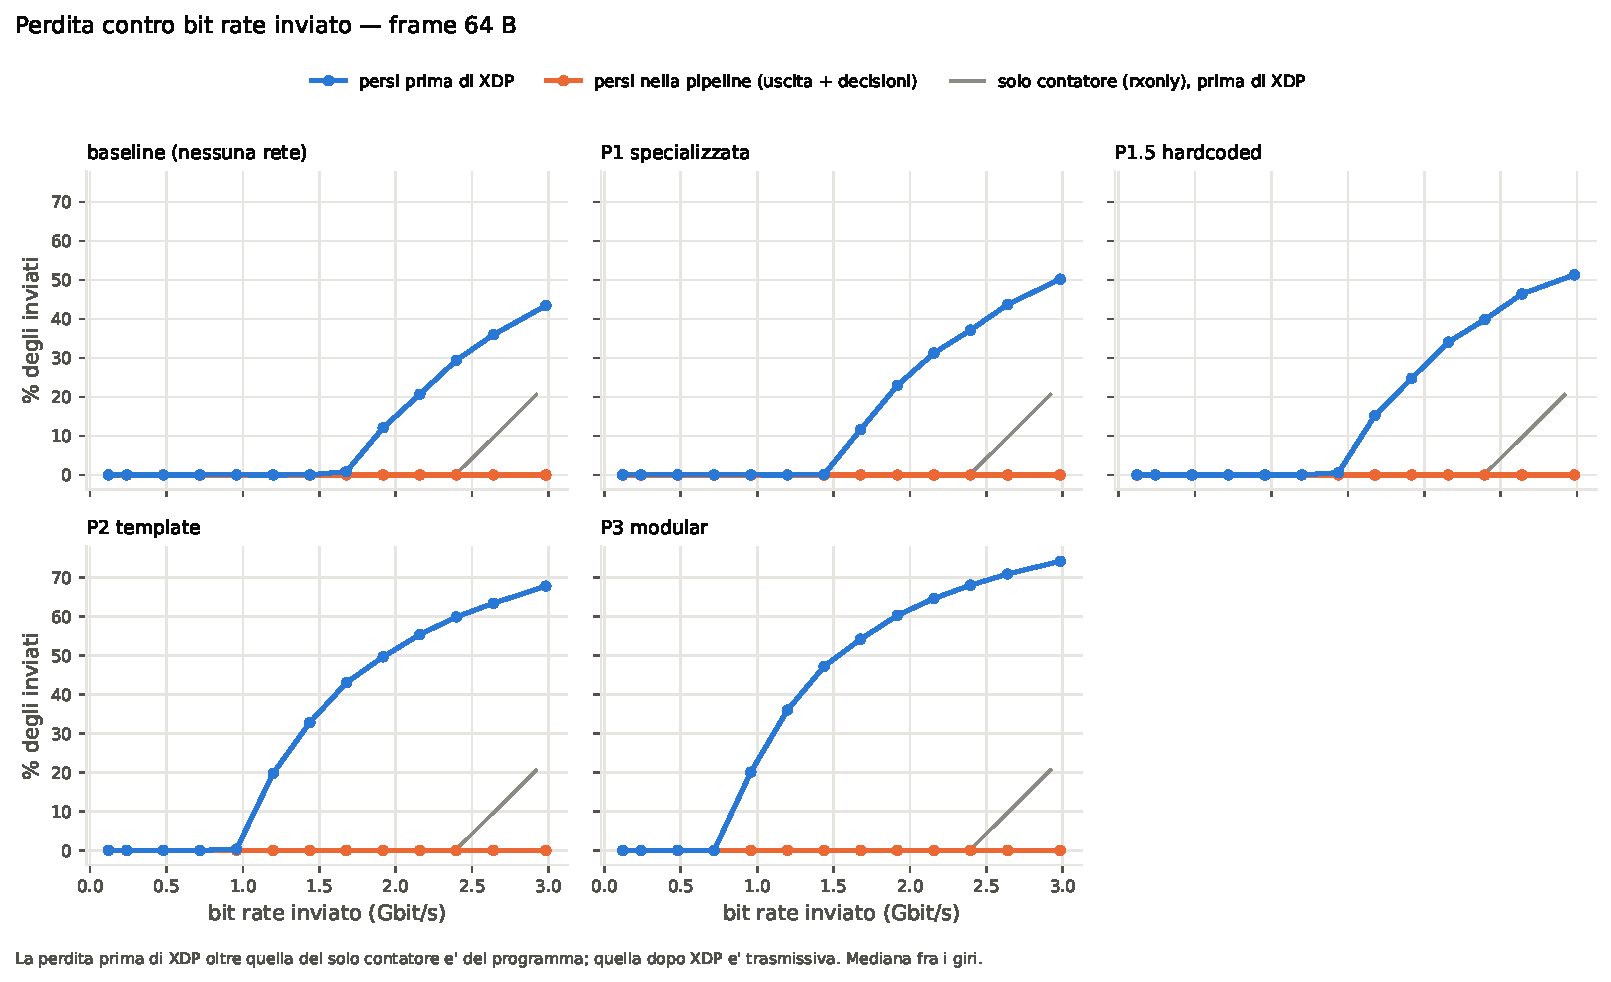
\includegraphics[width=\textwidth]{figures/bitrate_loss.pdf}
\end{center}

La stessa cosa come perdita: la curva dei persi prima di XDP sale, quella dei
persi dentro la pipeline o all'uscita resta a zero, al massimo lo 0,04\% degli
inviati. Il solo contatore non perde fino a 11 milioni al secondo: la perdita
delle pipeline non è della ricezione ma del programma.

\begin{center}
\small
\begin{tabular}{@{}lrrr@{}}
\toprule
\textbf{Pipeline} & \textbf{pulita fino a} & \textbf{perde da} & \textbf{inoltro massimo} \\
\midrule
baseline   & 4,05 Gbit/s & ---$^*$ & 9,02$^*$ M/s \\
P1 statica & 4,04 & 4,56 & 8,66 \\
P1.5       & 4,08 & 4,56 & 8,17 \\
P2         & 1,54 & 1,79 & 3,45 \\
P3         & 1,02 & 1,28 & 2,37 \\
\bottomrule
\end{tabular}\\[2pt]
{\footnotesize\color{soft} pacchetti da 64 byte; bit rate misurato sul collegamento; nodo su un P-core.
$^*$ baseline: oltre 8 M/s il limite è del banco, non del programma}
\end{center}

Le prime due colonne sono \textbf{gradini}, non soglie esatte: ``pulita fino a
1,54, perde da 1,79'' vuol dire che la perdita comincia da qualche parte fra i
due. Esempio: P2 inoltra al massimo 3,45 milioni di pacchetti al secondo, cioè
$3{,}45\cdot10^6 \times 64 \times 8 \approx 1{,}77$~Gbit/s, proprio fra i due
gradini.

\subsection*{Il ritardo}

\begin{center}
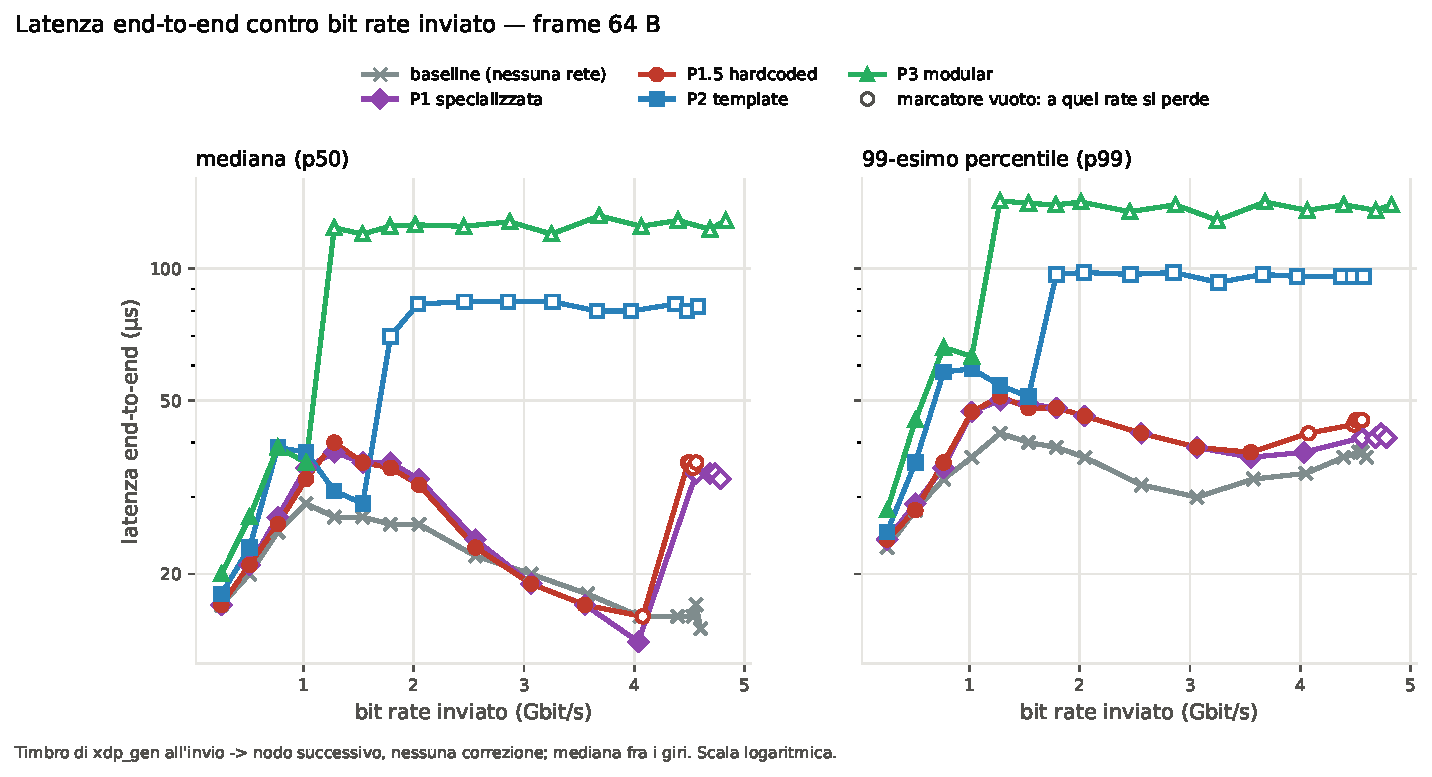
\includegraphics[width=\textwidth]{figures/bitrate_latency.pdf}
\end{center}

Il ritardo fa quello che la domanda prevede: resta di qualche decina di
microsecondi finché il nodo regge, poi \textbf{salta} esattamente dove la pipeline
comincia a perdere (marcatori vuoti), e da lì resta piatto. Il salto è la coda
d'ingresso che si riempie: 256 posti davanti a un programma che serve un
pacchetto ogni 117~ns (P1), 124 (P1.5), 290 (P2) o 425 (P3) fanno 30, 32, 74 e
109 microsecondi di attesa; le curve si fermano a circa 35, 36, 82 e 122~µs, e il
resto è il percorso fino al nodo successivo. La baseline non riempie mai la
coda. Oltre, la coda non può crescere: è piena, e ciò che arriva in più viene
respinto. Il ritardo si ferma e cresce la perdita. A basso carico la mediana
contiene l'attesa nel generatore (sezione~\ref{sec:limiti}, punto 5).

\subsection*{Perché il collo di bottiglia è il programma}

È quello che ci si deve aspettare, per come funziona XDP. Il programma non ha una
coda sua: gira dall'inizio alla fine su ogni pacchetto, sul core che riceve, e
finché non ha finito quel core non prende il pacchetto successivo. Se i pacchetti
arrivano più in fretta di quanto il core li finisca, si accumulano nella coda
\emph{davanti} al programma, e quando è piena vengono respinti. La perdita
all'ingresso è quindi il segno di un nodo più lento del traffico, e il nodo è il
suo programma.

Resta da escludere che il limite sia la sola ricezione, che gira sullo stesso
core. Lo dice \texttt{rxonly}, il contatore da solo: fino a 11 milioni di
pacchetti al secondo \textbf{non perde niente}, perché la sola ricezione regge
circa 19 milioni. Al traffico più alto P1 perde il 7\%, P1.5 il 9\%, P2 il 63\%,
P3 il 76\%: la perdita è del programma, e cresce con il suo costo. L'uscita invece
non limita: dopo il programma si perde lo 0,04\% al massimo, ed è rumore di
lettura.

Due precisazioni. Per la baseline il ``programma'' è quasi solo lettura
dell'intestazione e redirect: il suo limite è il costo fisso di un nodo XDP, non
una rete neurale. E il nodo ha \textbf{una sola coda e un solo core} per scelta,
per misurare il costo per core: una scheda di rete vera distribuisce i pacchetti
su più code e più core (RSS), e la capacità del nodo cresce con il numero di
core, mentre il costo per pacchetto resta quello misurato qui.

\section{Due core}
\label{sec:duecore}

Perché la capacità cresca davvero con i core, i core non devono contendersi
niente di scritto a ogni pacchetto. Per questo i contatori delle pipeline
(pacchetti inoltrati, persi, scartati, e uno per classe) sono \textbf{per-core}:
ogni core incrementa la sua copia, senza istruzioni atomiche, e chi legge somma
le copie. E ogni core del nodo ha la sua coda d'ingresso, il suo thread di
\texttt{xdp\_gen}, la sua coda d'uscita e il suo core d'uscita: il cavo virtuale
sceglie la coda d'uscita dal numero del core che inoltra, e con una coda sola i
due core del nodo scriverebbero nello stesso anello, svuotato da un solo core
del nodo successivo (l'esempio della sezione~\ref{sec:limiti}, punto 2).

\begin{center}
\small
\begin{tabular}{@{}lrrrrrr@{}}
\toprule
& \multicolumn{3}{c}{\textbf{P-core}} & \multicolumn{3}{c}{\textbf{E-core}} \\
\cmidrule(lr){2-4}\cmidrule(lr){5-7}
\textbf{Programma} & \textbf{1 core} & \textbf{2 core} & \textbf{del doppio}
& \textbf{1 core} & \textbf{2 core} & \textbf{del doppio} \\
\midrule
baseline & 15,27 & 29,11 & 95\%  & 9,39 & 19,09 & 102\% \\
P1       & 8,56  & 17,46 & 102\% & 6,35 & 12,74 & 100\% \\
P1.5     & 8,04  & 16,19 & 101\% & 5,84 & 11,71 & 100\% \\
P2       & 3,45  & 6,63  & 96\%  & 2,83 & 5,60  & 99\% \\
P3       & 2,36  & 4,60  & 98\%  & 1,94 & 3,84  & 99\% \\
\bottomrule
\end{tabular}\\[2pt]
{\footnotesize\color{soft} Milioni di pacchetti elaborati al secondo,
alimentatore. Due P-core: 6 e 8, uscite su 3 e 5. Due E-core: 12 e 16, uno per
modulo, uscite su 6 e 8.}
\end{center}

Con due core ogni programma elabora il doppio (95--102\%): il secondo core non
rallenta il primo, e il costo per core è quello di un core solo entro una decina
di nanosecondi. Per un nodo con $N$ code vale quindi $N$ volte la capacità
misurata su un core, finché generatore e scheda reggono.

\begin{lezione}
Per tutte e cinque la perdita è \textbf{all'ingresso}: il collo di bottiglia è il
programma eBPF, non la trasmissione, e la sola ricezione non perde affatto. Il
ritardo cresce fino a una perdita, come previsto, e si ferma al livello della coda
piena.
\end{lezione}

\section{Il nodo sui core lenti}
\label{sec:corelenti}

Il processore del portatile ha tre tipi di core: sei \textbf{P-core} veloci
(Redwood Cove), otto \textbf{E-core} efficienti (Crestmont, in due moduli da
quattro che dividono la cache L2 e la frequenza) e due \textbf{LP E-core}, che
stanno su un'altra parte del chip, fuori dalla cache L3. Che cosa succede se il
nodo gira su un core lento?

Per rispondere cambia \emph{solo} il core del nodo. Generatore e nodo successivo
restano su P-core a 3,5~GHz, così il generatore satura sempre il nodo e l'uscita
non diventa il collo di bottiglia. L'E-core gira anche lui a 3,5~GHz (il suo
massimo è 3,8): a parità di frequenza, la differenza di capacità è tutta nel
numero di cicli per pacchetto. Il LP E-core gira al suo massimo, 2,5~GHz. Gli
altri tre core del modulo dell'E-core restano a riposo: dividono con lui cache e
frequenza.

\begin{center}
\small
\begin{tabular}{@{}lrrrrrr@{}}
\toprule
& \multicolumn{3}{c}{\textbf{milioni di pacchetti/s}} & \textbf{E/P} &
\textbf{istruzioni} & \textbf{IPC} \\
\cmidrule(lr){2-4}
\textbf{Pipeline} & \textbf{P-core} & \textbf{E-core} & \textbf{LP E-core} & &
\textbf{per pacchetto} & \textbf{P / E / LP E} \\
\midrule
baseline & 15,27 & 9,39 & 3,29$^*$ & 0,61 & 606     & 2,7 / 1,7 / 0,8 \\
P1       & 8,56  & 6,35 & 3,10     & 0,74 & 1\,220  & 3,0 / 2,3 / 1,5 \\
P1.5     & 8,04  & 5,84 & 2,91     & 0,73 & 1\,426  & 3,3 / 2,4 / 1,7 \\
P2       & 3,45  & 2,83 & 1,57     & 0,82 & 4\,556  & 4,5 / 3,7 / 2,9 \\
P3       & 2,36  & 1,94 & 1,10     & 0,82 & 6\,573  & 4,4 / 3,7 / 2,9 \\
\bottomrule
\end{tabular}\\[2pt]
{\footnotesize\color{soft} Tre giri, alimentatore, 64 byte. Le istruzioni per
pacchetto sono le stesse sui tre tipi di core entro il 2\%. $^*$ Sul LP E-core
la baseline non satura (nodo al 93\%): il generatore non riesce a offrire di
più, e la cifra è un limite inferiore.}
\end{center}

\begin{lezione}
Il codice eseguito è lo stesso su ogni core: \textbf{cambia l'IPC}, cioè quante
istruzioni il core completa per ciclo. E non cambia allo stesso modo per tutte
le pipeline.
\end{lezione}

L'E-core rallenta soprattutto la \textbf{parte fissa} del nodo: ricevere il
pacchetto dalla coda, inoltrarlo, restituire la pagina. È lavoro del kernel, con
salti e accessi alla memoria, e l'E-core lo fa a IPC 1,7 invece di 2,7: la
baseline costa 106~ns invece di 66, il 60\% in più. L'aritmetica della rete
neurale, invece, è una fila di moltiplicazioni senza bivi, e l'E-core la esegue
quasi altrettanto bene (IPC 3,7 contro 4,4 per P3): l'inferenza di P3 sopra la
baseline costa 409~ns invece di 359, solo il 14\% in più. Per questo il rapporto
di capacità sale con il peso della pipeline: 0,61 per la baseline, 0,82 per P2
e P3.

Il LP E-core paga anche la memoria: sta fuori dalla L3, e i pacchetti scritti
dal generatore gli arrivano da lontano, con 14--19 mancate dell'ultimo livello
di cache per pacchetto (zero sugli altri core). Fra la frequenza più bassa e
l'IPC più basso regge dal 36 al 47\% del P-core sulle pipeline.

\begin{prima}[Esempio: la saturazione sull'E-core]
Le curve del bit rate sull'E-core hanno la stessa forma di quelle del P-core:
inoltro pieno fino alla capacità, poi piatto, perdita sempre all'ingresso. Il
ginocchio sta più in basso: 6,2 milioni al secondo per P1, 5,8 per P1.5, 2,8 per
P2, 1,9 per P3. E a coda piena il ritardo è più lungo, perché ogni pacchetto
costa di più: 45~µs per P1, 148 per P3.
\end{prima}

\section{Gli assi sotto traffico vero}
\label{sec:assireali}

Le analisi del capitolo sul costo che cresce --- larghezza, profondità, pesi
fermi, pesi a zero --- sono fatte con il programma da solo. Lo stesso banco di
questo capitolo le rifà con traffico vero: diciotto modelli sintetici, uno per
punto, con lo stesso descrittore del modello depositato, sul P-core e
sull'E-core.

\begin{center}
\small
\begin{tabular}{@{}lrrrrrr@{}}
\toprule
\textbf{strati da 4 neuroni} & 1 & 2 & 3 & 4 & 5 & 6 \\
\midrule
P1   & 113 & 116 & 119 & 124 & 125 & 132 \\
P1.5 & 121 & 128 & 131 & 132 & 134 & 138 \\
P2   & 264 & 287 & 329 & 344 & 368 & 396 \\
P3   & 351 & 421 & 486 & 545 & 595 & 652 \\
\midrule
P3, istruzioni per pacchetto & 5\,488 & 6\,576 & 7\,663 & 8\,759 & 9\,856 & 10\,952 \\
\bottomrule
\end{tabular}\\[2pt]
{\footnotesize\color{soft} Nanosecondi di CPU per pacchetto, nodo su un P-core;
la baseline resta a 64--67~ns in ogni punto.}
\end{center}

Gli andamenti sono quelli del programma da solo, più il costo fisso del nodo.
P3 paga circa 60~ns per strato, e i contatori hardware dicono perché: ogni
strato aggiunge \textbf{esattamente 1\,096 istruzioni eseguite}, su P-core e su
E-core. Sono le letture che ricostruiscono il contesto a ogni rientro, sempre le
stesse. A pesi fermi P2 sale del 35\% e P3 del 60\% da uno a cinque strati,
mentre le P1 restano fra 125 e 135~ns; con il 90\% dei pesi a zero P1 passa da
113 a 95~ns e P1.5 da 120 a 106, mentre P2 e P3 non si muovono, con le stesse
istruzioni. Sull'E-core ogni punto costa il 20--35\% in più.

\paragraph{La sola rete neurale.} Il tempo di CPU contiene anche il costo fisso
del nodo. Per isolare la rete neurale si usano le tre marcature della build
strumentata: T2$-$T1, meno la stessa misura della baseline, con il traffico a
0,3 e 0,6 milioni di pacchetti al secondo. Il \textbf{minimo} per finestra,
cioè il pacchetto che trova tutto in cache, coincide con il programma da solo:
P3 da 1 a 6 strati 262 $\rightarrow$ 508~ns contro 246 $\rightarrow$ 510. La
\textbf{media}, il costo tipico, sta sopra di 10--40~ns per P1 e P1.5 e di
40--110~ns per P2 e P3 (P3 a 6 strati 610~ns), con gli stessi andamenti su
ogni asse; sull'E-core lo scarto è circa doppio. Sul modello depositato la
media sopra la baseline (P1 44, P2 229, P3 364~ns) coincide con il tempo di CPU
meno la baseline (51, 224, 359): due misure indipendenti dello stesso costo.

\begin{center}
\small
\begin{tabular}{@{}lrrrrrr@{}}
\toprule
\textbf{strati da 4 neuroni} & 1 & 2 & 3 & 4 & 5 & 6 \\
\midrule
P2, da solo      & 157 & 179 & 206 & 227 & 256 & 286 \\
P2, media T2$-$T1 & 214 & 252 & 264 & 267 & 324 & 356 \\
P3, da solo      & 246 & 303 & 356 & 408 & 453 & 510 \\
P3, media T2$-$T1 & 322 & 348 & 436 & 509 & 560 & 610 \\
\bottomrule
\end{tabular}\\[2pt]
{\footnotesize\color{soft} Nanosecondi di rete neurale per pacchetto (baseline
sottratta), nodo su un P-core. Da solo: \texttt{BPF\_PROG\_TEST\_RUN}, minimo
su 7 prove.}
\end{center}

\paragraph{La rete e l'ingresso.} Con una rete diversa per punto, da 10 a 100
nodi, il costo della rete neurale (tempo di CPU meno la baseline) resta piatto
su tutte le pipeline: P1 45--52~ns, P2 221--237, P3 351--366, con le stesse
istruzioni eseguite. Lo stesso per una one-hot d'ingresso da 16 a 65 colonne;
gli ingressi densi invece costano (da 5 a 17 colonne P3 sale di 72~ns). Contando
le moltiplicazioni davvero eseguite, ingressi densi, one-hot e larghezza cadono
su una retta: circa 0,2~ns per moltiplicazione con i pesi compilati e 0,7~ns
per P3 ($r^2$ 0,71--0,94); P2 no, perché il suo costo di partenza cambia con
la composizione dell'ingresso.

\section{Che cosa questo numero non dice}

I limiti del banco sono nella sezione \ref{sec:limiti}. Uno in più riguarda il
modello:

\begin{itemize}
  \item \textbf{Modelli sintetici sugli assi.} Sul traffico vero il modello
        depositato è misurato in ogni configurazione; le variazioni di forma
        (sezione~\ref{sec:assireali}) usano modelli sintetici con lo stesso
        descrittore, un giro di tre misure per punto.
  \item \textbf{Due tipi di core lenti, a una frequenza.} L'E-core è misurato a
        3,5~GHz, non al suo massimo di 3,8; il LP E-core solo al suo massimo.
\end{itemize}

% ==================================================================
\chapter{La macchina di laboratorio, sotto controllo}
\label{ch:macchina}
% ==================================================================

Tutte le misure di questo quaderno sono fatte sulla macchina di laboratorio,
senza strati di mezzo: un portatile Lenovo IdeaPad Slim 5 con un \textbf{Intel
Core Ultra 7 155H}, Ubuntu 24.04 installato direttamente sul disco (dual boot),
kernel 6.8. Questo capitolo spiega che cosa serve perché le misure si ripetano.

\section{Un processore che non sta fermo}

Il 155H è \textbf{ibrido}: tre tipi di core diversi sullo stesso chip.

\begin{center}
\small
\begin{tabular}{@{}llll@{}}
\toprule
\textbf{tipo} & \textbf{CPU} & \textbf{frequenza} & \textbf{note} \\
\midrule
P-core (prestazioni) & 0--11 & base 1,4, turbo 4,5--4,8 GHz & 6 core fisici, due thread ciascuno \\
E-core (efficienza) & 12--19 & base 0,9, turbo 3,8 GHz & \\
LP E-core & 20--21 & base 0,7, turbo 2,5 GHz & fuori dalla cache condivisa \\
\bottomrule
\end{tabular}
\end{center}

Lasciato a sé stesso, un banco su questa macchina finisce dove capita: una
regola generica per scegliere i processori (un terzo al nodo, il resto al
generatore) darebbe quattordici thread di generatore e metterebbe il nodo sui
core di efficienza, e il desktop girerebbe sul gemello del core misurato. La
frequenza va da 0,4 a 4,8~GHz secondo il carico, e i core si addormentano in uno
stato da cui il risveglio costa 310 microsecondi: più di quanto la coda
d'ingresso da 256 posti copra a un milione di pacchetti al secondo.

E il portatile \textbf{scalda}. Un solo P-core salito a 4,5--4,8~GHz porta il
processore da 51 a 99~°C in due secondi, e il chip riduce la frequenza per
difendersi (\emph{throttling}).

\section{Le condizioni, messe e tolte}

\texttt{ipa/test/host\_conditions.py} mette la macchina in condizioni note per la
durata di un banco, e le riporta com'erano alla fine.

\begin{itemize}
  \item \textbf{Ruoli}: nodo, nodo successivo e generatore su core fisici
        \emph{diversi}, un thread per core; il gemello di ciascuno resta a riposo;
        il core della CPU~0 resta al sistema. Qui: nodo sulla CPU~6, nodo
        successivo sull'8, generatore sulla 10. Quando il nodo va su un E-core
        (la 12) restano a riposo anche gli altri tre core del suo modulo (13--15),
        che dividono con lui la cache L2 e la frequenza.
  \item \textbf{Frequenza fissa} sui core del banco (governor \emph{performance},
        minimo uguale al massimo), e \textbf{misurata} dai contatori del processore
        (APERF/MPERF).
  \item \textbf{Tetto sui core del sistema} (2,5~GHz): il turbo del desktop
        scalderebbe il chip fino a rallentare anche i core del banco.
  \item \textbf{Niente sonno profondo} sui core del banco: spenti gli stati con
        risveglio oltre un microsecondo.
  \item \textbf{Isolamento}: desktop, servizi, interruzioni e thread del kernel
        spostabili confinati sulle CPU del sistema.
  \item \textbf{Frequenza della cache condivisa fissa}, profilo energetico
        \emph{performance}, watchdog spento.
\end{itemize}

Ogni valore si salva \emph{prima} di cambiarlo, in un file in memoria. A fine run
--- anche con Ctrl-C o un errore --- si riscrive tutto all'indietro; un run ucciso
lascia il file, e il run successivo ripristina per primo. Un test sul kernel vero
(\texttt{test\_host\_kernel.py}, 25 controlli) applica le condizioni, le rilegge
dal kernel, verifica che un processo del desktop giri solo sulle CPU del sistema,
misura la frequenza sotto carico, ripristina e confronta la macchina valore per
valore con com'era --- anche dopo aver ucciso il processo a condizioni applicate.

Durante ogni misura un \textbf{monitor} legge gli interventi di throttling, la
temperatura, la frequenza vera del nodo e le interruzioni del firmware. Una
finestra misurata fuori dalle condizioni dichiarate viene marcata e contata, non
scartata in silenzio.

\section{La frequenza scritta non è la frequenza vera}

La frequenza \emph{base} del processore, 1,4~GHz, è l'unica garantita. Il sistema
la accetta e la rilegge: 1\,400 minimo, 1\,400 massimo. I contatori del
processore dicono un'altra cosa:

\begin{lezione}
Con 1\,400~MHz scritti nel sistema, il core gira a \textbf{circa 2\,000~MHz} ---
fisso e stabile, ma non a quella frequenza. Da 3\,000~MHz in su scritto e vero
coincidono entro 10~MHz.
\end{lezione}

Se il monitor si fidasse del numero scritto, a 1,4~GHz marcherebbe come
disturbate 38 finestre su 39. La frequenza di riferimento è quindi quella
\textbf{misurata} all'avvio, su ogni core del banco; il numero scritto resta
accanto, per confronto.

\section{Quale frequenza}

Più alta la frequenza, più alto il throughput --- finché il portatile regge. La
risposta si è misurata, con un giro corto di \texttt{bench\_bitrate} per frequenza
e due run completi di cinque minuti:

\begin{center}
\small
\begin{tabular}{@{}ll@{}}
\toprule
\textbf{frequenza vera} & \textbf{macchina} \\
\midrule
2,0--3,5 GHz, 30 s & pulita \\
4,0 GHz, 30 s & pulita \\
4,5 GHz, 30 s & throttling su 28 finestre su 39 \\
4,0 GHz, run completo & fino a 98~°C, il core del nodo in throttling \\
3,5 GHz, run completo & massimo 85~°C, una finestra disturbata su 390 \\
\bottomrule
\end{tabular}
\end{center}

A 4,5~GHz il throughput smette di crescere: il chip si difende. A 4~GHz un run
corto è pulito, uno da cinque minuti porta il processore a 98~°C e il core del
nodo stesso in throttling. \textbf{3,5~GHz} è la frequenza più alta che la
macchina regge per un run intero, ed è la frequenza di default del banco.

\begin{lezione}
La frequenza pesa quasi in proporzione, ma non del tutto: da 3 a 4~GHz il
throughput sale del 23\% invece del 33\%, perché la cache condivisa e la memoria
non accelerano con il core. Quello che non si muove è il \textbf{rapporto fra
pipeline}. Le cifre assolute si citano con la loro frequenza, e con il tipo di
core (sezione~\ref{sec:corelenti}).
\end{lezione}

\section{Il risultato: misure che si ripetono}

\begin{center}
\small
\begin{tabular}{@{}lr@{}}
\toprule
\textbf{banco} & \textbf{variazione} \\
\midrule
programma da solo (\texttt{test\_suite}, fra sette prove) & 0--7\% \\
throughput a saturazione, quattro misure diverse della stessa sessione & entro il 2\% \\
inoltro allo stesso punto della curva (fra cinque giri) & in genere 0,1\% \\
\bottomrule
\end{tabular}
\end{center}

E i pacchetti respinti con il nodo sotto capacità sono \textbf{zero}: il core del
nodo non dorme, e nessun altro lavoro gli viene dato.

\section{Come si rifà tutto}

Uno script rifà ogni misura di questo quaderno, nelle stesse condizioni, in circa
un'ora. CSV, condizioni della macchina e registri vanno in
\texttt{results/campagna\_<data>/}, con una sintesi delle tabelle; i grafici del
quaderno si rigenerano in \texttt{docs/figures/}:

\begin{lstlisting}
bash ipa/test/remeasure_campagna.sh        # tutto: traffico su P-, E-, LP E-core, assi, kernel
bash ipa/test/remeasure_campagna.sh pcore  # solo una parte
bash ipa/test/remeasure_all.sh             # solo programma, correttezza, analisi parametrica
\end{lstlisting}

% ==================================================================
\chapter{Altri modelli, altre reti}
\label{ch:modelli}
% ==================================================================

\section{La domanda}

Quasi ogni numero dei capitoli precedenti viene da un modello solo, il 65-4-4-7
addestrato su Germany50. Un banco che funziona solo su quel modello potrebbe
avere la sua forma scritta dentro senza che nessuno se ne accorga: gli strati di
P3 elencati a mano, sei bit di stato dei link, il significato delle classi letto
sempre dalla scheda del checkpoint. Un modello diverso girerebbe allora con i
pesi, o con le classi, di un altro. L'obiettivo di questo capitolo: \textbf{lo
stesso test, per qualsiasi modello e qualsiasi rete}, e un errore chiaro quando
la combinazione non ha senso.

\section{Scenario e modello}

Le due parole hanno un significato preciso.

\begin{itemize}
  \item \textbf{Lo scenario è la rete}: quattro numeri in
        \texttt{topologies/<nome>/topology\_config.json}, cioè quante
        interfacce ha al massimo un nodo, quanti nodi ha la rete, quante code ha
        ogni interfaccia e con che TTL i pacchetti ci entrano.
  \item \textbf{Il modello è la rete neurale}: pesi, forma, ingressi (ognuno con
        la sua larghezza e la sua scala) e significato di ogni classe.
\end{itemize}

\begin{center}
\small
\begin{tabular}{@{}lrrrrp{4.6cm}@{}}
\toprule
\textbf{Scenario} & \textbf{interf.} & \textbf{nodi} & \textbf{code} & \textbf{TTL} & \textbf{modelli che ci girano} \\
\midrule
\texttt{germany50}       & 6 & 52  & 4 & 30 & checkpoint, ipa\_like, deep, sparse, sparse\_hetero\_11 \\
\texttt{germany50\_ttl16} & 6 & 52  & 4 & 16 & ipa\_ttl16 \\
\texttt{synth\_small}    & 3 & 8   & -- & 16 & small \\
\texttt{synth\_ones}     & 3 & 4   & -- & 8  & ones \\
\texttt{synth\_large}    & 8 & 100 & -- & 64 & large \\
\texttt{synth\_mixed}    & 4 & 12  & 1 & 30 & mixed \\
\bottomrule
\end{tabular}
\end{center}

Oltre a Germany50 ci sono le reti dei modelli sintetici. Non sono topologie
reali: sono le dimensioni per cui ciascun modello sintetico è stato generato.

\section{Quando un modello può girare su una rete}

Ogni ingresso del modello prende la sua larghezza da una dimensione della rete:
lo stato dei link e la porta d'ingresso dalle interfacce, l'identità del nodo
dai nodi, l'occupazione delle code dalle code. E il TTL il modello lo legge
diviso per il TTL iniziale con cui è stato addestrato
(sezione~\ref{sec:ttl} nel capitolo sulla matematica). Quindi:

\begin{lezione}
Un modello gira su una rete solo se \textbf{ogni suo ingresso è largo quanto la
dimensione della rete da cui dipende} e se \textbf{la scala del suo TTL è il TTL
iniziale della rete}.
\end{lezione}

Esempio: il checkpoint ha il one-hot del nodo largo 52. Su una rete da 30 nodi
metà delle sue colonne non corrisponderebbe a nessun nodo, e il test si ferma
subito con
\begin{lstlisting}
nodi: il modello ne vuole 52, la rete ne ha 30
\end{lstlisting}
Esempio con il TTL: \texttt{ipa\_ttl16} ha la stessa forma del checkpoint, ma è
addestrato con il TTL diviso per 16. Su Germany50, dove i pacchetti partono da
30, vedrebbe valori fino a quasi 2 invece che fino a 1, fuori da tutto ciò su
cui è stato addestrato. Per questo gira sulla sua rete, \texttt{germany50\_ttl16}.

C'è poi un secondo filtro, fra modello e \emph{pipeline}. Ogni pipeline ha dei
tetti fissati quando il programma viene compilato:
\begin{itemize}
  \item \textbf{P2}: al massimo 8 neuroni per strato, strati dal terzo in poi
        larghi come il secondo, 1\,024 pesi in tutto;
  \item \textbf{P3}: al massimo 8 neuroni per strato, 16 strati, 2\,048 pesi;
  \item \textbf{P1}: nessuno, perché il programma si genera per quel modello.
\end{itemize}
Il modello \texttt{large} (117-8-8-9) ha 1\,097 pesi e un primo strato da 117
per 8: P2 e P3 non lo possono caricare. Non è un errore del test: la
combinazione è \textbf{non applicabile}, ed è contata a parte.

\section{Come è costruito}

Quattro pezzi, ognuno con un compito solo.

\begin{enumerate}
  \item \texttt{model\_source.py} \textbf{carica qualsiasi modello nello stesso
        formato}: il checkpoint, un altro \texttt{.pt}, un preset sintetico
        (\texttt{synth:deep}) o una cartella. Il significato delle classi è
        quello che il modello dichiara. Contiene anche il controllo modello
        contro rete.
  \item \texttt{pipeline\_limits.py} \textbf{dice se una pipeline regge una
        forma}, con i numeri presi dai moduli che compilano i programmi, così i
        due non possono divergere.
  \item \texttt{pipeline\_setup.py} \textbf{carica un modello in una pipeline}:
        baseline, P1, P1.5, P2, P3. Sono gli stessi costruttori del confronto a
        tre vie.
  \item \texttt{model\_under\_test.py} \textbf{legge \texttt{--model} e
        \texttt{--topology}} e li passa ai processi figli con due variabili
        d'ambiente.
\end{enumerate}

Senza \texttt{--model} si usa il checkpoint; con \texttt{--model checkpoint} si
usa lo stesso checkpoint per la strada generica, e il risultato è identico
(sezione~\ref{sec:stradanuova}).

\begin{lstlisting}
sudo python3 ipa/test/test_suite.py --only kernel --model synth:deep
sudo python3 ipa/test/test_fabric.py --model synth:small
sudo python3 ipa/test/bench_throughput.py --mode compare --generator xdp --model synth:deep
sudo python3 ipa/test/bench_throughput.py --mode compare --generator xdp \
     --model ipa/synth/traffic/depth_3
\end{lstlisting}
Senza \texttt{--topology} viene scelta la rete compatibile (Germany50 se lo è).

\section{Che cosa controllano i test}

Passare un modello diverso chiede controlli precisi in tre punti.

\textbf{L'azione, non solo la classe.} Col checkpoint, fra TTL 2 e 6, la classe
è sempre un inoltro; un altro modello può decidere DROP proprio lì. Il test
controlla che il programma abbia scelto la classe del riferimento \emph{e} ne
abbia eseguito l'azione: redirect per un inoltro, \texttt{XDP\_DROP} per uno
scarto, \texttt{XDP\_PASS} per una classe inutilizzata.

\textbf{Tutte le classi che il modello sa decidere.} Il fabric cerca un caso per
ogni classe cambiando stato dei link e TTL; per le classi che così non trova
cambia anche porta d'ingresso, nodo e code, e ogni caso scrive i suoi valori
nelle mappe prima di spedire il pacchetto. Col checkpoint basta lo stato dei
link; coi pesi casuali dei sintetici conta anche il resto. Classi consegnate:

\begin{center}
\small
\begin{tabular}{@{}ll@{}}
\toprule
\textbf{Modello} & \textbf{classi consegnate} \\
\midrule
checkpoint & 0, 1, 2, 3, 4, 5 \\
ipa\_like, ipa\_ttl16 & 2, 3, 4, 5 \\
small, mixed & 0, 1, 2, 3 \\
large & 1, 4, 6, 8 \\
deep / sparse / ones & 0, 1, 4 / 1, 5 / 0 \\
\bottomrule
\end{tabular}
\end{center}
Le classi che mancano il modello non le decide mai: su 200\,000 ingressi casuali
\texttt{deep} sceglie solo 0, 1 e 4, e \texttt{ones}, che ha tutti i pesi uguali
a 1, sceglie sempre la classe 0. È una proprietà del modello, non un limite del
test.

\textbf{Il traffico misura un inoltro.} I generatori mandano pacchetti con TTL
32. Col checkpoint, con tutti i link attivi, quel pacchetto viene inoltrato; con
\texttt{large} invece viene scartato, e il banco misurerebbe lo scarto
chiamandolo inoltro. Il banco allora cerca lo stato dei link che porta a un
inoltro, lo scrive nella mappa e lo stampa:
\begin{lstlisting}
traffico di large con link_state=00111000, TTL 32 -> classe 4 (FORWARD)
\end{lstlisting}
Se nessuno stato dei link porta a un inoltro, la pipeline non si misura. Fra i
modelli degli assi sotto traffico (sezione~\ref{sec:assireali}) tre, con il
seme comune, decidevano lo scarto in tutti i 64 stati: il generatore dei modelli
fa lo stesso controllo e, in quei casi, passa al seme successivo.

\section{La prova che la strada generica non cambia niente}
\label{sec:stradanuova}

Il checkpoint passato esplicitamente, \texttt{--model checkpoint}, va per la
strada generica. Confrontato con il checkpoint senza \texttt{--model}:
\begin{itemize}
  \item pesi, scala e significato delle classi identici; il riferimento Python
        dà la stessa classe e lo stesso logit su 3\,000 ingressi;
  \item il sorgente di P1 e la foglia di P2 sono identici \emph{byte per byte};
  \item il riferimento generico coincide con quello scritto per il 65-4-4-7 su
        20\,000 ingressi.
\end{itemize}

E la correttezza sui modelli nuovi:
\begin{itemize}
  \item nel kernel, ogni scenario per ogni modello compatibile per ogni pipeline,
        40 ingressi a testa, sotto due identificativi di modello:
        \textbf{110 su 110}, più \texttt{large} non applicabile a P2 e P3;
  \item suite kernel su nove modelli: tutto PASS.
\end{itemize}

\section{I risultati}

Nel kernel, con \texttt{BPF\_PROG\_TEST\_RUN}, nanosecondi per pacchetto
(minimo su sette prove; baseline 14--15~ns ovunque):

\begin{center}
\small
\begin{tabular}{@{}llrrrr@{}}
\toprule
\textbf{Modello} & \textbf{forma} & \textbf{P1} & \textbf{P1.5} & \textbf{P2} & \textbf{P3} \\
\midrule
checkpoint & 65-4-4-7   & 46 & 51 & 197 & 318 \\
ipa\_like  & 65-4-4-7   & 47 & 51 & 194 & 309 \\
ipa\_ttl16 & 65-4-4-7   & 40 & 46 & 197 & 310 \\
sparse     & 65-4-4-7   & 31 & 38 & 197 & 314 \\
deep       & 65-4-4-4-7 & 52 & 56 & 226 & 375 \\
small      & 15-4-4     & 30 & 37 & 139 & 226 \\
mixed      & 18-6-5     & 36 & 43 & 155 & 257 \\
ones       & 11-2-3     & 23 & 28 & 129 & 217 \\
large      & 117-8-8-9  & 71 & 76 & --- & --- \\
\bottomrule
\end{tabular}
\end{center}

Tre cose si leggono subito.
\begin{itemize}
  \item \textbf{P2 e P3 costano per la forma, P1 per i valori dei pesi.}
        Checkpoint, \texttt{ipa\_like}, \texttt{ipa\_ttl16} e \texttt{sparse}
        hanno la stessa forma: P2 e P3 costano uguale per tutti (194--197 e
        309--318~ns), mentre P1 va da 31~ns (\texttt{sparse}, pesi a zero tolti
        in compilazione) a 47.
  \item \textbf{Uno strato in più costa a P2 e P3}: \texttt{deep} ha uno strato
        più del checkpoint e costa +29~ns su P2, +57~ns su P3, +6~ns su P1.
  \item \textbf{Ingressi più piccoli abbassano P2 e P3} di 40--100~ns: il primo
        strato, che è il più largo, scorre meno colonne.
\end{itemize}

Sul traffico vero gli stessi effetti --- profondità, larghezza, pesi a zero ---
sono misurati sugli assi, con diciotto modelli sintetici dal descrittore del
checkpoint (sezione~\ref{sec:assireali}).

\begin{lezione}
Il confronto fra le pipeline non è una proprietà del checkpoint: su nove
modelli l'ordine P1 $<$ P1.5 $<$ P2 $<$ P3 resta lo stesso, e i costi si spostano
come ci si aspetta dalla forma. La profondità pesa su P2 e P3, l'ampiezza
dell'ingresso su tutte, e su P1 più che altrove.
\end{lezione}

\section{Che cosa non fa}

\begin{itemize}
  \item \textbf{Nessun modello sintetico è addestrato}: servono a provare le
        pipeline su forme diverse, non a dire qualcosa sull'instradamento.
\end{itemize}

% ==================================================================
\chapter{I numeri in una pagina}
\label{ch:numeri}
% ==================================================================

\begin{center}
\small
\begin{tabular}{@{}p{5.2cm}rrrrr@{}}
\toprule
& \textbf{baseline} & \textbf{P1 statica} & \textbf{P1.5} & \textbf{P2} & \textbf{P3} \\
\midrule
\multicolumn{6}{@{}l}{\emph{Il nodo su traffico vero, un P-core (capitolo \ref{ch:reale}), 64 byte}} \\
milioni di pacchetti al secondo & 15,27 & 8,56 & 8,04 & 3,45 & 2,36 \\
ns di CPU per pacchetto & 66 & 117 & 124 & 290 & 425 \\
costo della rete (sopra la baseline) & --- & 51 ns & 58 ns & 224 ns & 359 ns \\
istruzioni eseguite per pacchetto & 606 & 1\,220 & 1\,426 & 4\,556 & 6\,573 \\
istruzioni per ciclo & 2,7 & 3,0 & 3,3 & 4,5 & 4,4 \\
pulita fino a (bit rate) & $\geq$ 4,05 & 4,04 & 4,08 & 1,54 & 1,02 Gbit/s \\
\addlinespace
\multicolumn{6}{@{}l}{\emph{Lo stesso nodo su un E-core e su un LP E-core}} \\
milioni di pacchetti al secondo, E-core & 9,39 & 6,35 & 5,84 & 2,83 & 1,94 \\
\quad rispetto al P-core & 0,61 & 0,74 & 0,73 & 0,82 & 0,82 \\
milioni di pacchetti al secondo, LP E-core & $\geq$ 3,29 & 3,10 & 2,91 & 1,57 & 1,10 \\
\addlinespace
\multicolumn{6}{@{}l}{\emph{Il solo programma}} \\
$T_2-T_1$ sul percorso vero (minimo) & 26 ns & 60 ns & 69 ns & 216 ns & 331 ns \\
\texttt{BPF\_PROG\_TEST\_RUN}, pesi del modello & 14 ns & 46 ns & 52 ns & 194 ns & 318 ns \\
istruzioni del programma caricato & 135 & 606 & 1\,019 & 15\,089 & 12\,288 \\
\addlinespace
\multicolumn{6}{@{}l}{\emph{Cambiare modello su un nodo in servizio}} \\
caricare sul nodo & --- & \multicolumn{2}{c}{0,4--2,2 ms (AOT)} & \multicolumn{2}{c}{10--12 ms} \\
anche generare e compilare & --- & \multicolumn{2}{c}{57--121 ms} & \multicolumn{2}{c}{non serve} \\
serve un compilatore sul nodo? & --- & \multicolumn{2}{c}{no (compilato prima)} & \multicolumn{2}{c}{no} \\
\bottomrule
\end{tabular}\\[2pt]
{\footnotesize\color{soft} Campagna del 6 ottobre (\texttt{results/campagna\_2026-10-06/}),
core del banco a 3,5~GHz (2,5 il LP E-core). Il bit rate si misura su una griglia di
valori: ``pulita fino a'' è l'ultimo punto della griglia senza perdite, non la
capacità esatta.}
\end{center}

\begin{lezione}
In quattro righe:
\begin{enumerate}
  \item \textbf{Scrivere i pesi nel programma costa circa 50--60~ns per
        pacchetto sul nodo; leggerli da una tabella 225--360~ns.} È il prezzo della
        configurabilità.
  \item \textbf{Con l'oggetto precompilato, cambiare modello costa pochi
        millisecondi per tutte le pipeline}. Il vantaggio residuo di P2 e P3 è non
        dover compilare niente, da nessuna parte.
  \item \textbf{Congelare anche il nodo (P1 statica) vale poco ma si vede}: circa
        7~ns sul percorso vero, 5--7~ns sul solo programma, e la dimensione non
        dipende più dalla taglia della rete.
  \item \textbf{Su un core lento il codice è lo stesso, l'IPC no}: un E-core regge
        dal 61\% (baseline) all'82\% (P2, P3) del P-core, perché rallenta
        soprattutto la parte fissa del nodo e poco l'aritmetica della rete.
\end{enumerate}
\end{lezione}

% ==================================================================
\chapter{Quel che resta aperto}

\begin{itemize}
\item \textbf{Il costo del nodo di baseline e \texttt{rxonly}} con pacchetti
      grezzi: con un thread per coda il generatore non le satura sul P-core, e
      più thread intralciano la coda (sezione~\ref{sec:scrittore}); sul LP E-core
      il generatore non satura nemmeno la baseline. Serve un generatore più
      veloce su un solo scrittore, o una scheda vera.
\item \textbf{Tre marcature e latenza minima su modelli diversi}: solo col
      checkpoint (capitolo \ref{ch:modelli}).
\item \textbf{Gli E-core al loro massimo}, 3,8~GHz: misurati solo a 3,5.
\item \textbf{Hardware vero}: una scheda di rete con XDP nativo e una seconda
      macchina, per un numero che non sia di un cavo virtuale.
\item \textbf{Il tetto sull'uscita di P2}: lo strato finale è srotolato a 32
      classi per un modello che ne ha 7. Abbassarlo ridurrebbe il programma ma
      \emph{restringe l'insieme dei modelli rappresentabili}.
\item \textbf{I salti fra programmi di P3}: tre per pacchetto, ed è lì (con le
      letture che li accompagnano, 1\,096 istruzioni per strato) che sta la
      latenza.
\item \textbf{La profondità massima di P2} fra 20 e 37 strati: il punto esatto in
      cui clang si ferma non è misurato.
\item \textbf{Isolamento dal boot}: i core del banco sono isolati a sistema acceso;
      l'isolamento completo (tick e callback del kernel) richiede parametri di
      avvio.
\end{itemize}

% ==================================================================
\chapter{I comandi}

Tutti i comandi si lanciano dalla radice del repository. \texttt{sudo} serve
ovunque si carichi un programma nel kernel o si tocchi un'interfaccia; senza
\texttt{sudo} girano solo le prove che non escono da Python.

\begin{prima}[Prerequisiti]
Linux con BCC installato; per l'oggetto AOT di P1 anche
\begin{lstlisting}
sudo apt install clang libbpf-dev libelf-dev zlib1g-dev libzstd-dev liblzma-dev
\end{lstlisting}
Il generatore (\texttt{xdp\_gen}) è uno script del repository; il modulo
\texttt{pktgen}, per l'alternativa, il banco lo carica da sé.
\end{prima}

\section{La macchina}

\begin{lstlisting}
# topologia, piano dei ruoli e condizioni attuali (niente root)
python3 ipa/test/host_conditions.py --show

# un comando qualunque sul core del nodo, a condizioni applicate
sudo python3 ipa/test/host_conditions.py --run -- CMD ...

# se un run e' stato ucciso: rimette la macchina com'era
sudo python3 ipa/test/host_conditions.py --restore

# le condizioni verificate: su un /sys finto, e sul kernel vero
python3 ipa/test/test_host_conditions.py
sudo python3 ipa/test/test_host_kernel.py --bench

# tutte le misure del quaderno (circa un'ora)
bash ipa/test/remeasure_campagna.sh
\end{lstlisting}

\section{Correttezza: il modello fa quello che deve}

\begin{lstlisting}
python3 ipa/test/test_suite.py
python3 ipa/test/test_class_semantics.py
python3 ipa/test/test_synth.py
python3 ipa/test/verify_synth_kernel.py --all --dry-run
\end{lstlisting}

\section{Kernel: si carica, e quanto costa}

\begin{lstlisting}
sudo python3 ipa/test/host_conditions.py --run -- \
     python3 ipa/test/test_suite.py --only kernel
sudo python3 ipa/test/verify_multi_model.py
sudo python3 ipa/test/verify_per_model_semantics.py
sudo python3 ipa/test/verify_synth_kernel.py --all --n 300
sudo python3 ipa/test/verify_synth_kernel.py --all --n 300 --pipeline p2
sudo python3 ipa/test/verify_synth_kernel.py --all --n 300 --pipeline p3
\end{lstlisting}

\section{Altri modelli, altre reti}

\begin{lstlisting}
python3 ipa/test/test_model_source.py
sudo python3 ipa/test/test_model_source.py --kernel
sudo python3 ipa/test/host_conditions.py --run -- \
     python3 ipa/test/test_suite.py --only kernel --model synth:deep
sudo python3 ipa/test/test_fabric.py --model synth:small -q
python3 ipa/test/traffic_models.py          # i modelli degli assi sotto traffico
\end{lstlisting}

\section{Datapath reale: il pacchetto attraversa davvero}

\begin{lstlisting}
sudo python3 ipa/test/test_fabric.py
sudo python3 ipa/test/test_fabric.py --method aot
sudo python3 ipa/test/test_fabric.py --sweep
sudo python3 ipa/test/netns_fabric.py --cleanup
\end{lstlisting}

\section{Analisi parametrica: come cresce il costo}

\begin{lstlisting}
sudo python3 ipa/test/host_conditions.py --run -- \
     python3 ipa/test/bench_scaling.py --axis all --out results/
sudo python3 ipa/test/host_conditions.py --run -- \
     python3 ipa/test/bench_scaling.py --axis campaign --out results/
python3 ipa/test/bench_scaling.py --plot results/
sudo python3 ipa/test/bench_scaling.py --verify
sudo python3 ipa/test/bench_scaling.py --verify-ports
sudo python3 ipa/test/host_conditions.py --run -- \
     python3 ipa/test/bench_depth_vs_width.py
\end{lstlisting}

\section{Il test reale}

\begin{lstlisting}
# tutto il traffico: P-core, E-core, LP E-core, assi; poi la sintesi
bash ipa/test/remeasure_campagna.sh pcore ecore lpe assi
python3 ipa/test/campaign_report.py results/campagna_2026-10-06

# capacita' a un core: nodo su un P-core (6) o su un E-core (12)
sudo python3 ipa/test/bench_throughput.py --mode compare --generator xdp \
     --rounds 3 --gen-cpus 10 --dut-cpus 6 --egress-cpu 8 --out results/pcore
sudo python3 ipa/test/bench_throughput.py --mode compare --generator xdp \
     --rounds 3 --gen-cpus 10 --dut-cpus 12 --egress-cpu 8 --out results/ecore

# il bit rate crescente: latenza, ricevuti, inoltrati, dove si perde
sudo python3 ipa/test/bench_bitrate.py --generator xdp --gen-cpus 10 \
     --dut-cpus 6 --egress-cpu 8 --out results/bitrate
python3 ipa/test/bench_bitrate.py --report results/bitrate

# le tre marcature T1/T2/T3 su una scala di rate
sudo python3 ipa/test/bench_throughput.py --mode rates --generator xdp \
     --gen-cpus 10 --dut-cpus 6 --frames 64 --rounds 3 --rates 0.05,0.5,1,1.5,2,2.5,3

# per classe e per taglia
sudo python3 ipa/test/bench_throughput.py --mode compare --generator xdp \
     --gen-cpus 10 --dut-cpus 6 --egress-cpu 8 --per-class --rounds 3
sudo python3 ipa/test/bench_throughput.py --mode compare --generator xdp \
     --gen-cpus 10 --dut-cpus 6 --egress-cpu 8 --frames 64,512,1514 --rounds 3

# i contatori hardware, a mano
sudo python3 ipa/test/hw_counters.py --cpu 6,12,20 --seconds 1

# la finestra di misura e le formule, verificate senza kernel
python3 ipa/test/test_steady_window.py
python3 ipa/test/test_bitrate_math.py

# se un run si interrompe e lascia il generatore configurato
sudo python3 ipa/test/bench_throughput.py --cleanup
\end{lstlisting}

\begin{prima}[Come si legge l'uscita]
\textbf{Condizioni del test} --- in testa, e in \texttt{env.csv}: ruoli, frequenza
scritta e misurata, temperatura, interventi di throttling durante il run.

\textbf{Controllo di validità} --- la baseline deve essere la più veloce entro il
10\% e \texttt{rxonly} non deve essere più lento della baseline. Se una delle due
cose non vale, il run misura il banco e non le pipeline.

\textbf{Finestre marcate} --- «macchina» (fuori dalle condizioni dichiarate),
«raffica» o «gen» (il generatore non ha offerto il carico chiesto): contate e
riportate, non scartate.
\end{prima}

\section{Costi specifici e oggetto precompilato}

\begin{lstlisting}
sudo python3 ipa/test/bench_tailcall_overhead.py
python3 ipa/methods/method4_hardcoded_aot.py --build-only   # build, come utente
sudo python3 ipa/methods/method4_hardcoded_aot.py           # verifica e bench
sudo python3 ipa/test/diag_verifier.py                      # statistiche del verificatore
\end{lstlisting}

\section{L'ordine consigliato}

Partendo da zero su una macchina nuova:

\begin{enumerate}
\item \texttt{python3 ipa/test/host\_conditions.py --show} --- com'è fatta la
      macchina, e dove andrebbe il banco?
\item \texttt{python3 ipa/test/test\_synth.py} --- il C generato per P1 calcola il modello? (\texttt{test\_suite.py}, che controlla estrazione dei pesi e quantizzazione, richiede PyTorch)
\item \texttt{sudo python3 ipa/test/test\_host\_kernel.py} --- le condizioni si
      mettono e si tolgono davvero?
\item \texttt{sudo python3 ipa/test/test\_fabric.py} --- il pacchetto attraversa
      davvero?
\item \texttt{bash ipa/test/remeasure\_campagna.sh} --- tutti i numeri.
\end{enumerate}

\end{document}
